% ============================================================
% SECCIÓN: DISEÑO DEL SISTEMA
% Incluye todos los diagramas UML del sistema
% ============================================================

\newpage
\section{DISEÑO DEL SISTEMA}

Esta sección presenta el diseño detallado del sistema mediante diagramas UML que describen las funcionalidades disponibles para los usuarios y la arquitectura técnica interna del sistema.

\subsection{Diagramas de casos de uso}

Los diagramas de casos de uso describen las funcionalidades del sistema desde la perspectiva de los usuarios, identificando los actores que interactúan con el sistema y las acciones que pueden realizar. El sistema define tres roles principales: Administrador, Cajero y Usuario de Inventario.

El módulo de autenticación (Figura \ref{fig:cu-auth}) permite a todos los usuarios del sistema iniciar y cerrar sesión, recuperación de contraseles, y gestión de perfiles. Los administradores tienen privilegios adicionales para registrar nuevos usuarios.

\begin{figure}[H]
	\centering
	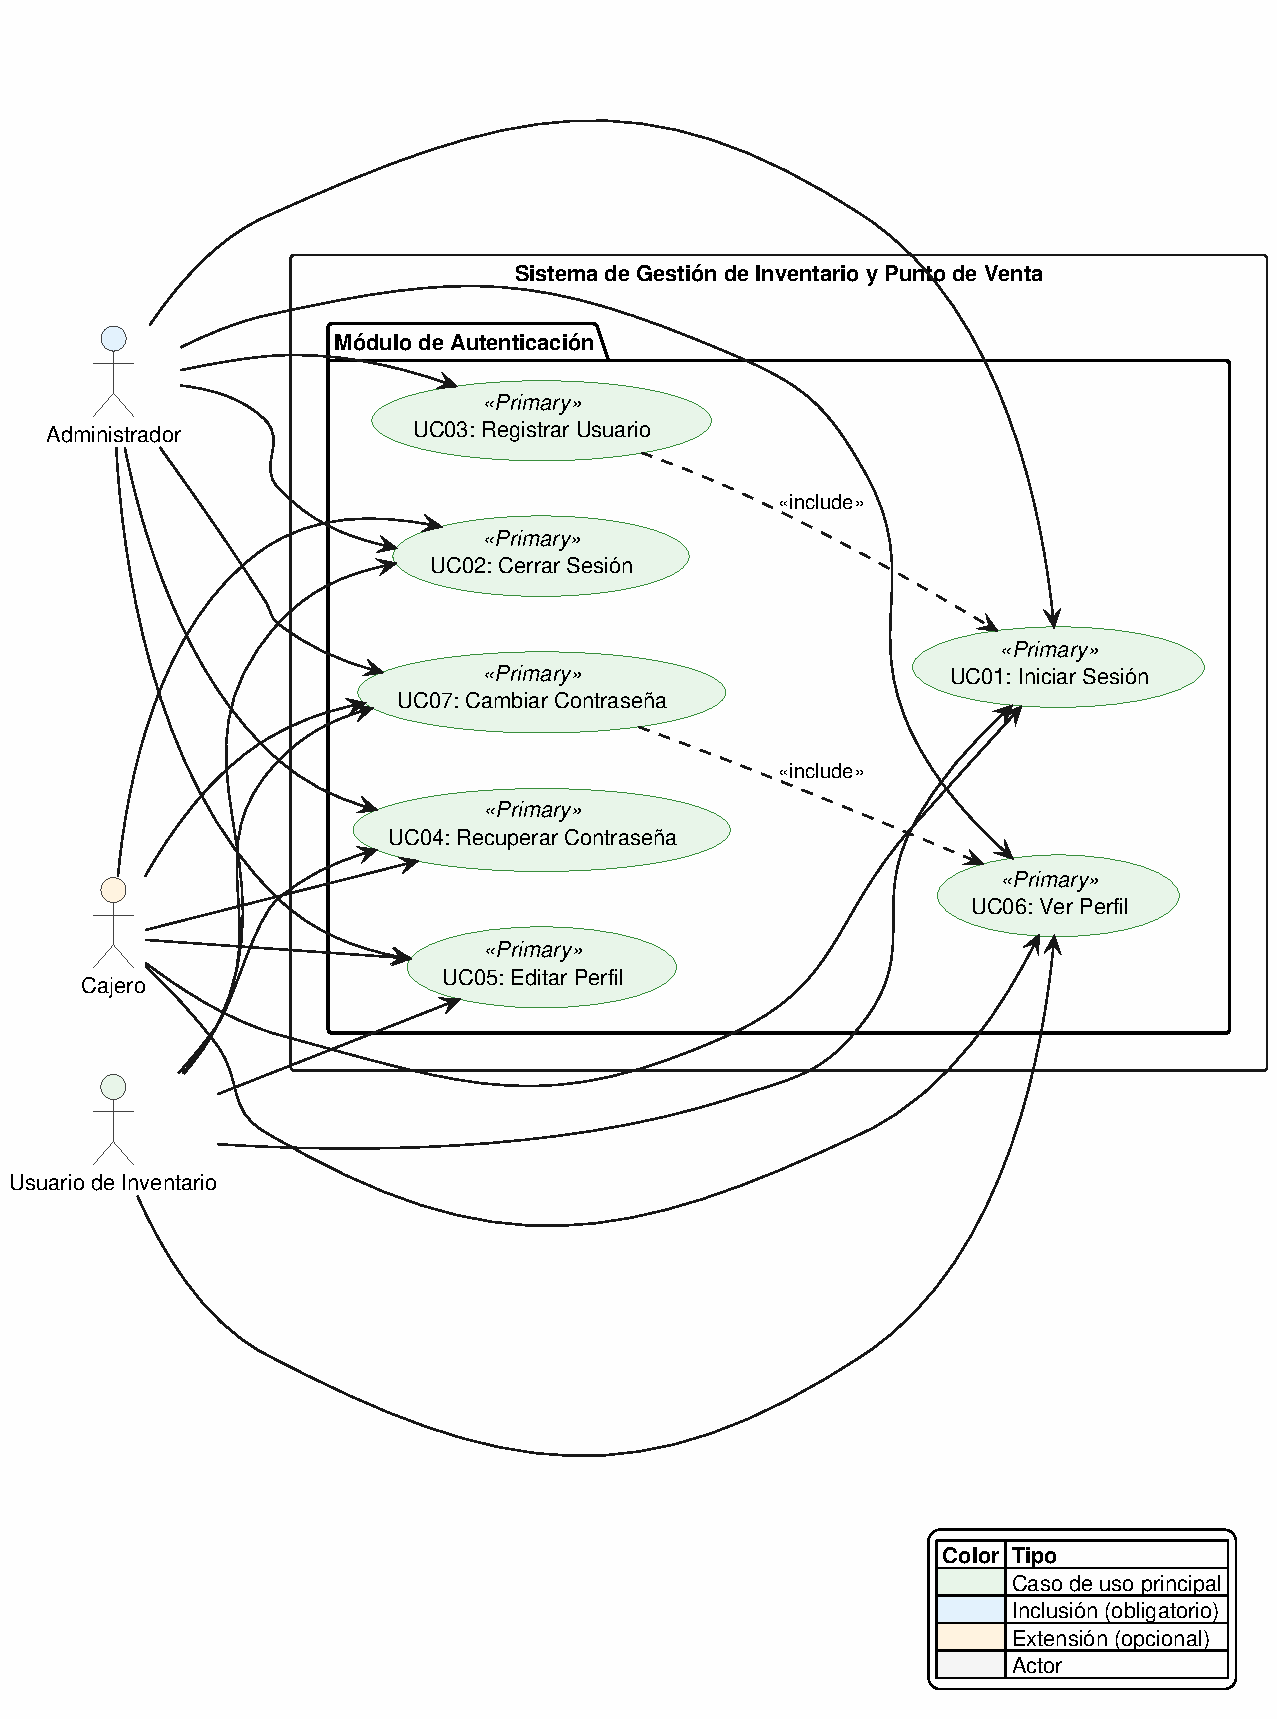
\includegraphics[width=0.9\textwidth]{Images/diagramas-uml/casos-de-uso/modulo-auth}
	\caption{Diagrama de casos de uso - Módulo de autenticación}
	\label{fig:cu-auth}
\end{figure}

El módulo de productos (Figura \ref{fig:cu-productos}) permite la gestión completa del inventario. Los administradores y usuarios de inventario pueden crear, editar, eliminar y consultar productos, gestionar categorías, controlar niveles de stock, y recibir alertas de stock bajo.

\begin{figure}[H]
	\centering
	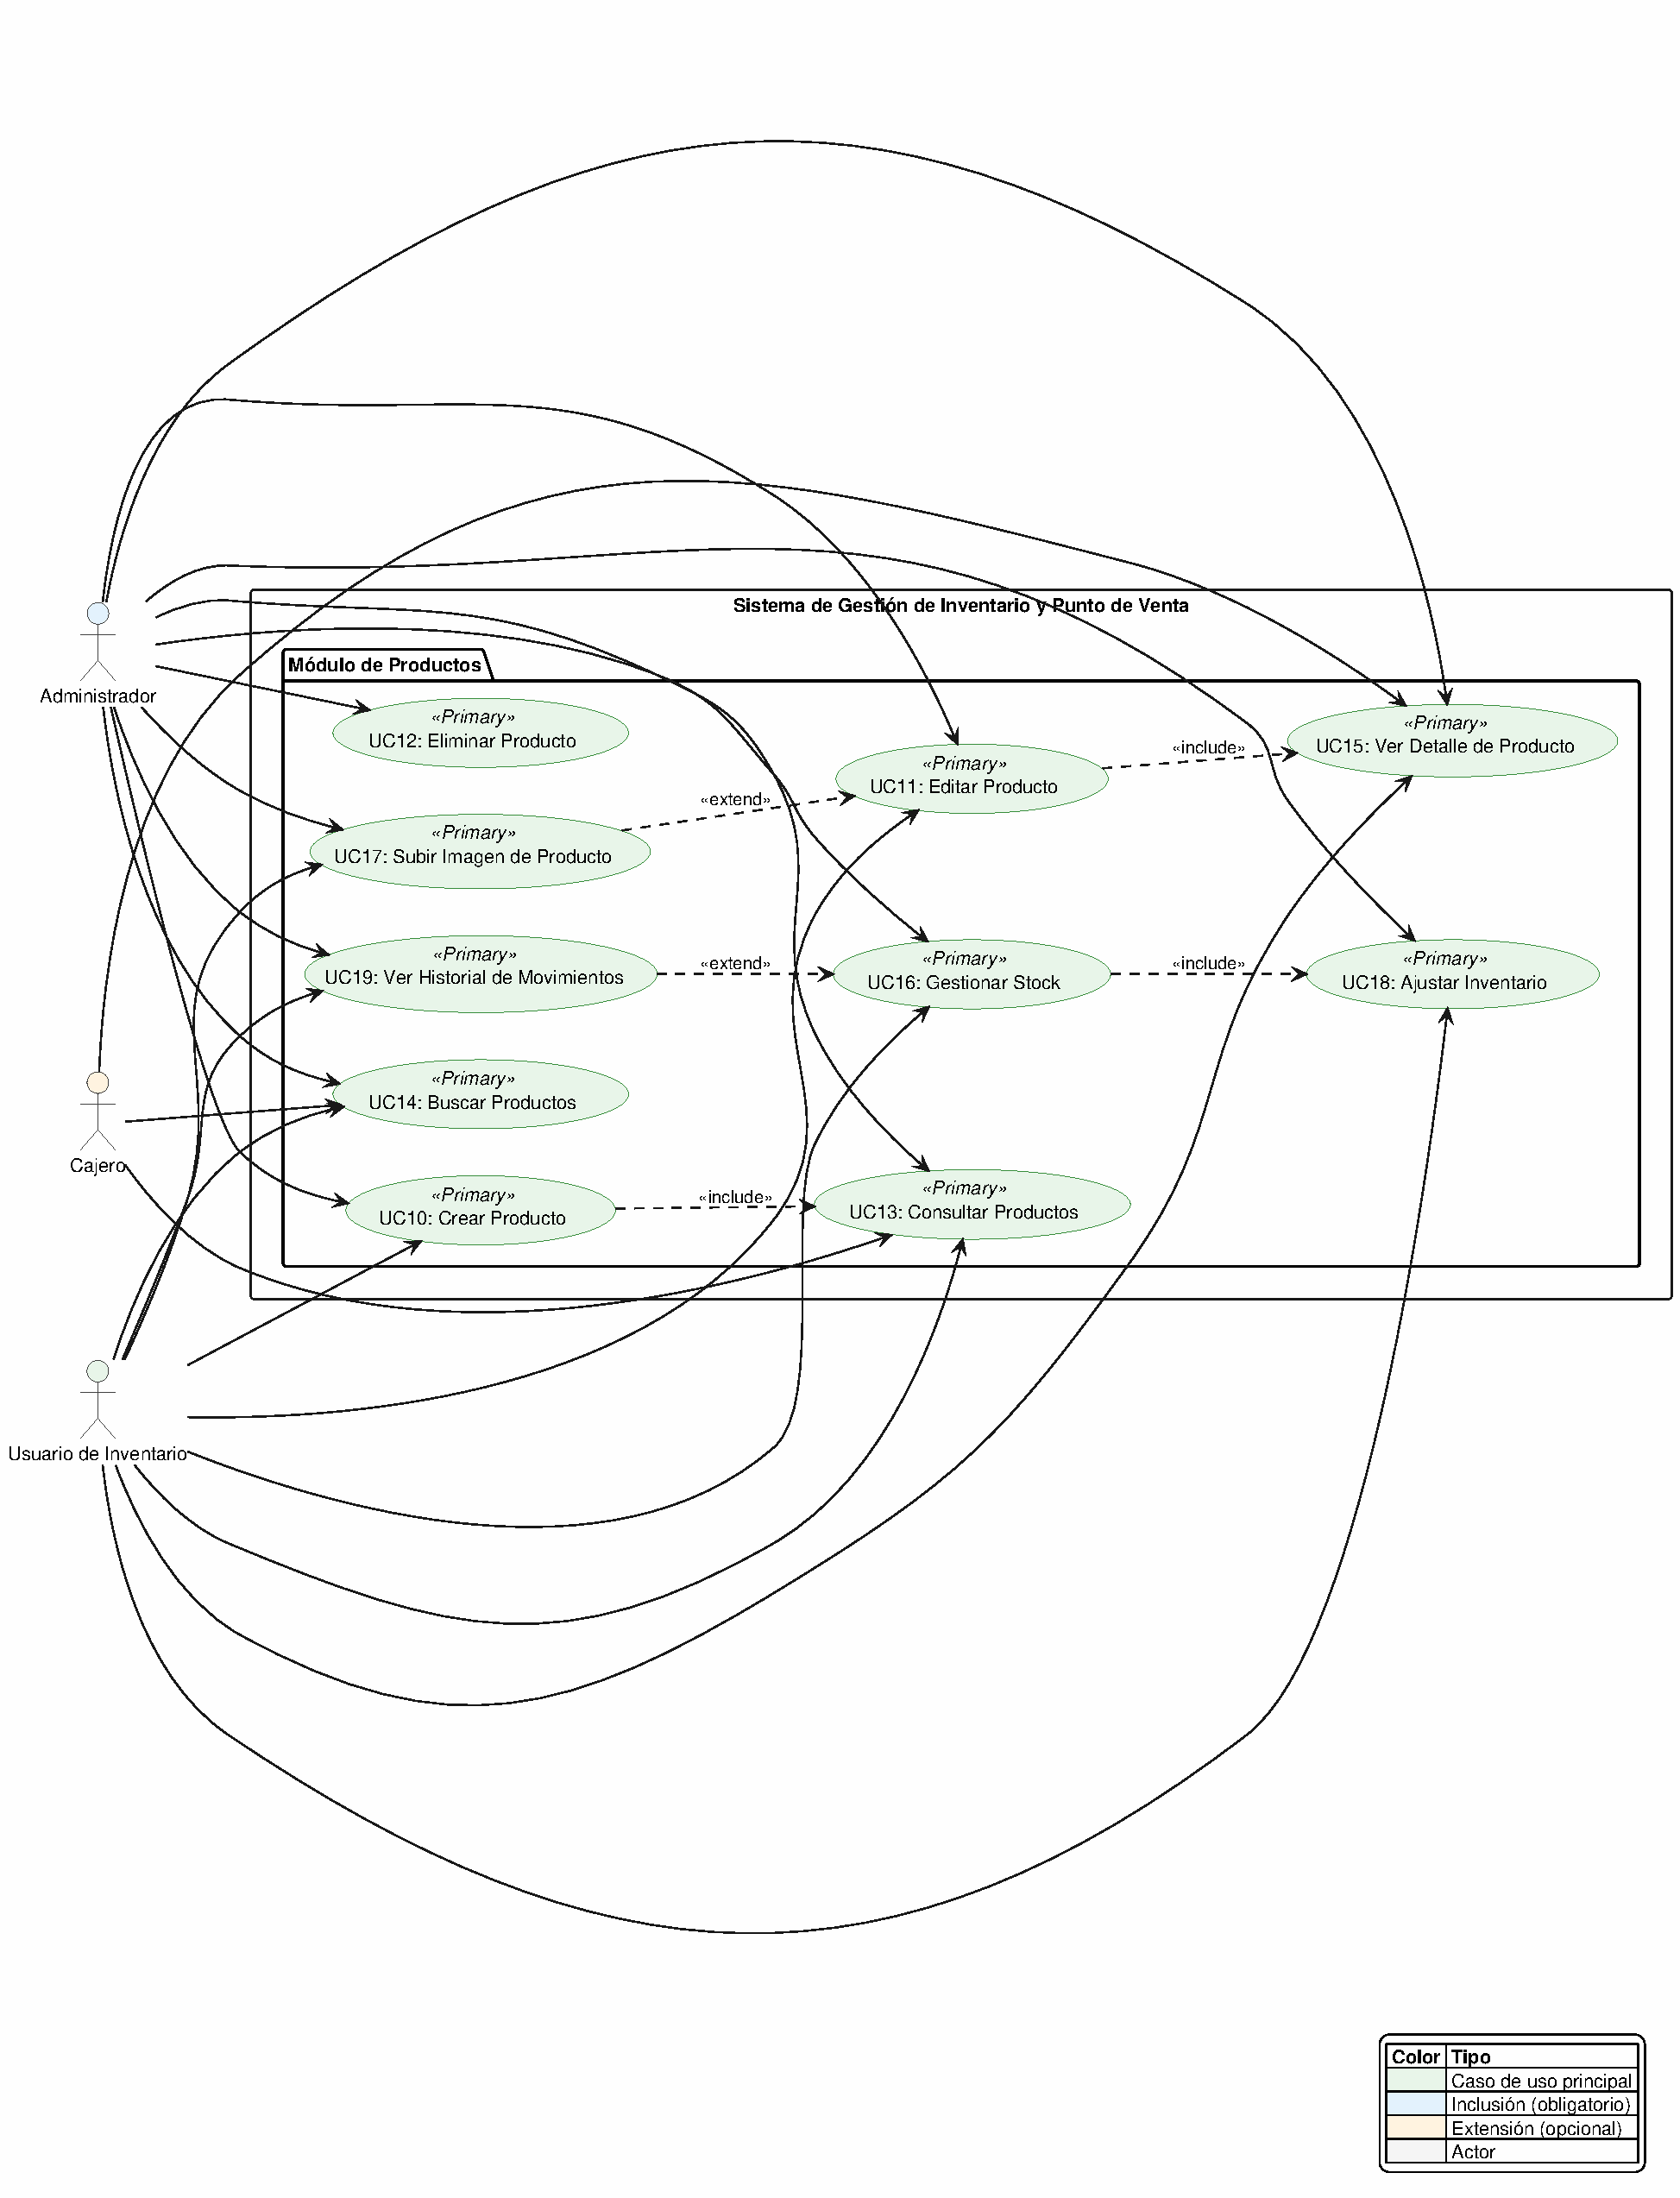
\includegraphics[width=0.9\textwidth]{Images/diagramas-uml/casos-de-uso/modulo-productos}
	\caption{Diagrama de casos de uso - Módulo de productos}
	\label{fig:cu-productos}
\end{figure}

El módulo de ventas (Figura \ref{fig:cu-ventas}) representa el punto de venta (POS) del sistema. Los cajeros pueden procesar ventas, pausar y reanudar transacciones, gestionar métodos de pago, y generar comprobantes. Los administradores pueden además cancelar ventas y acceder a reportes detallados.

\begin{figure}[H]
	\centering
	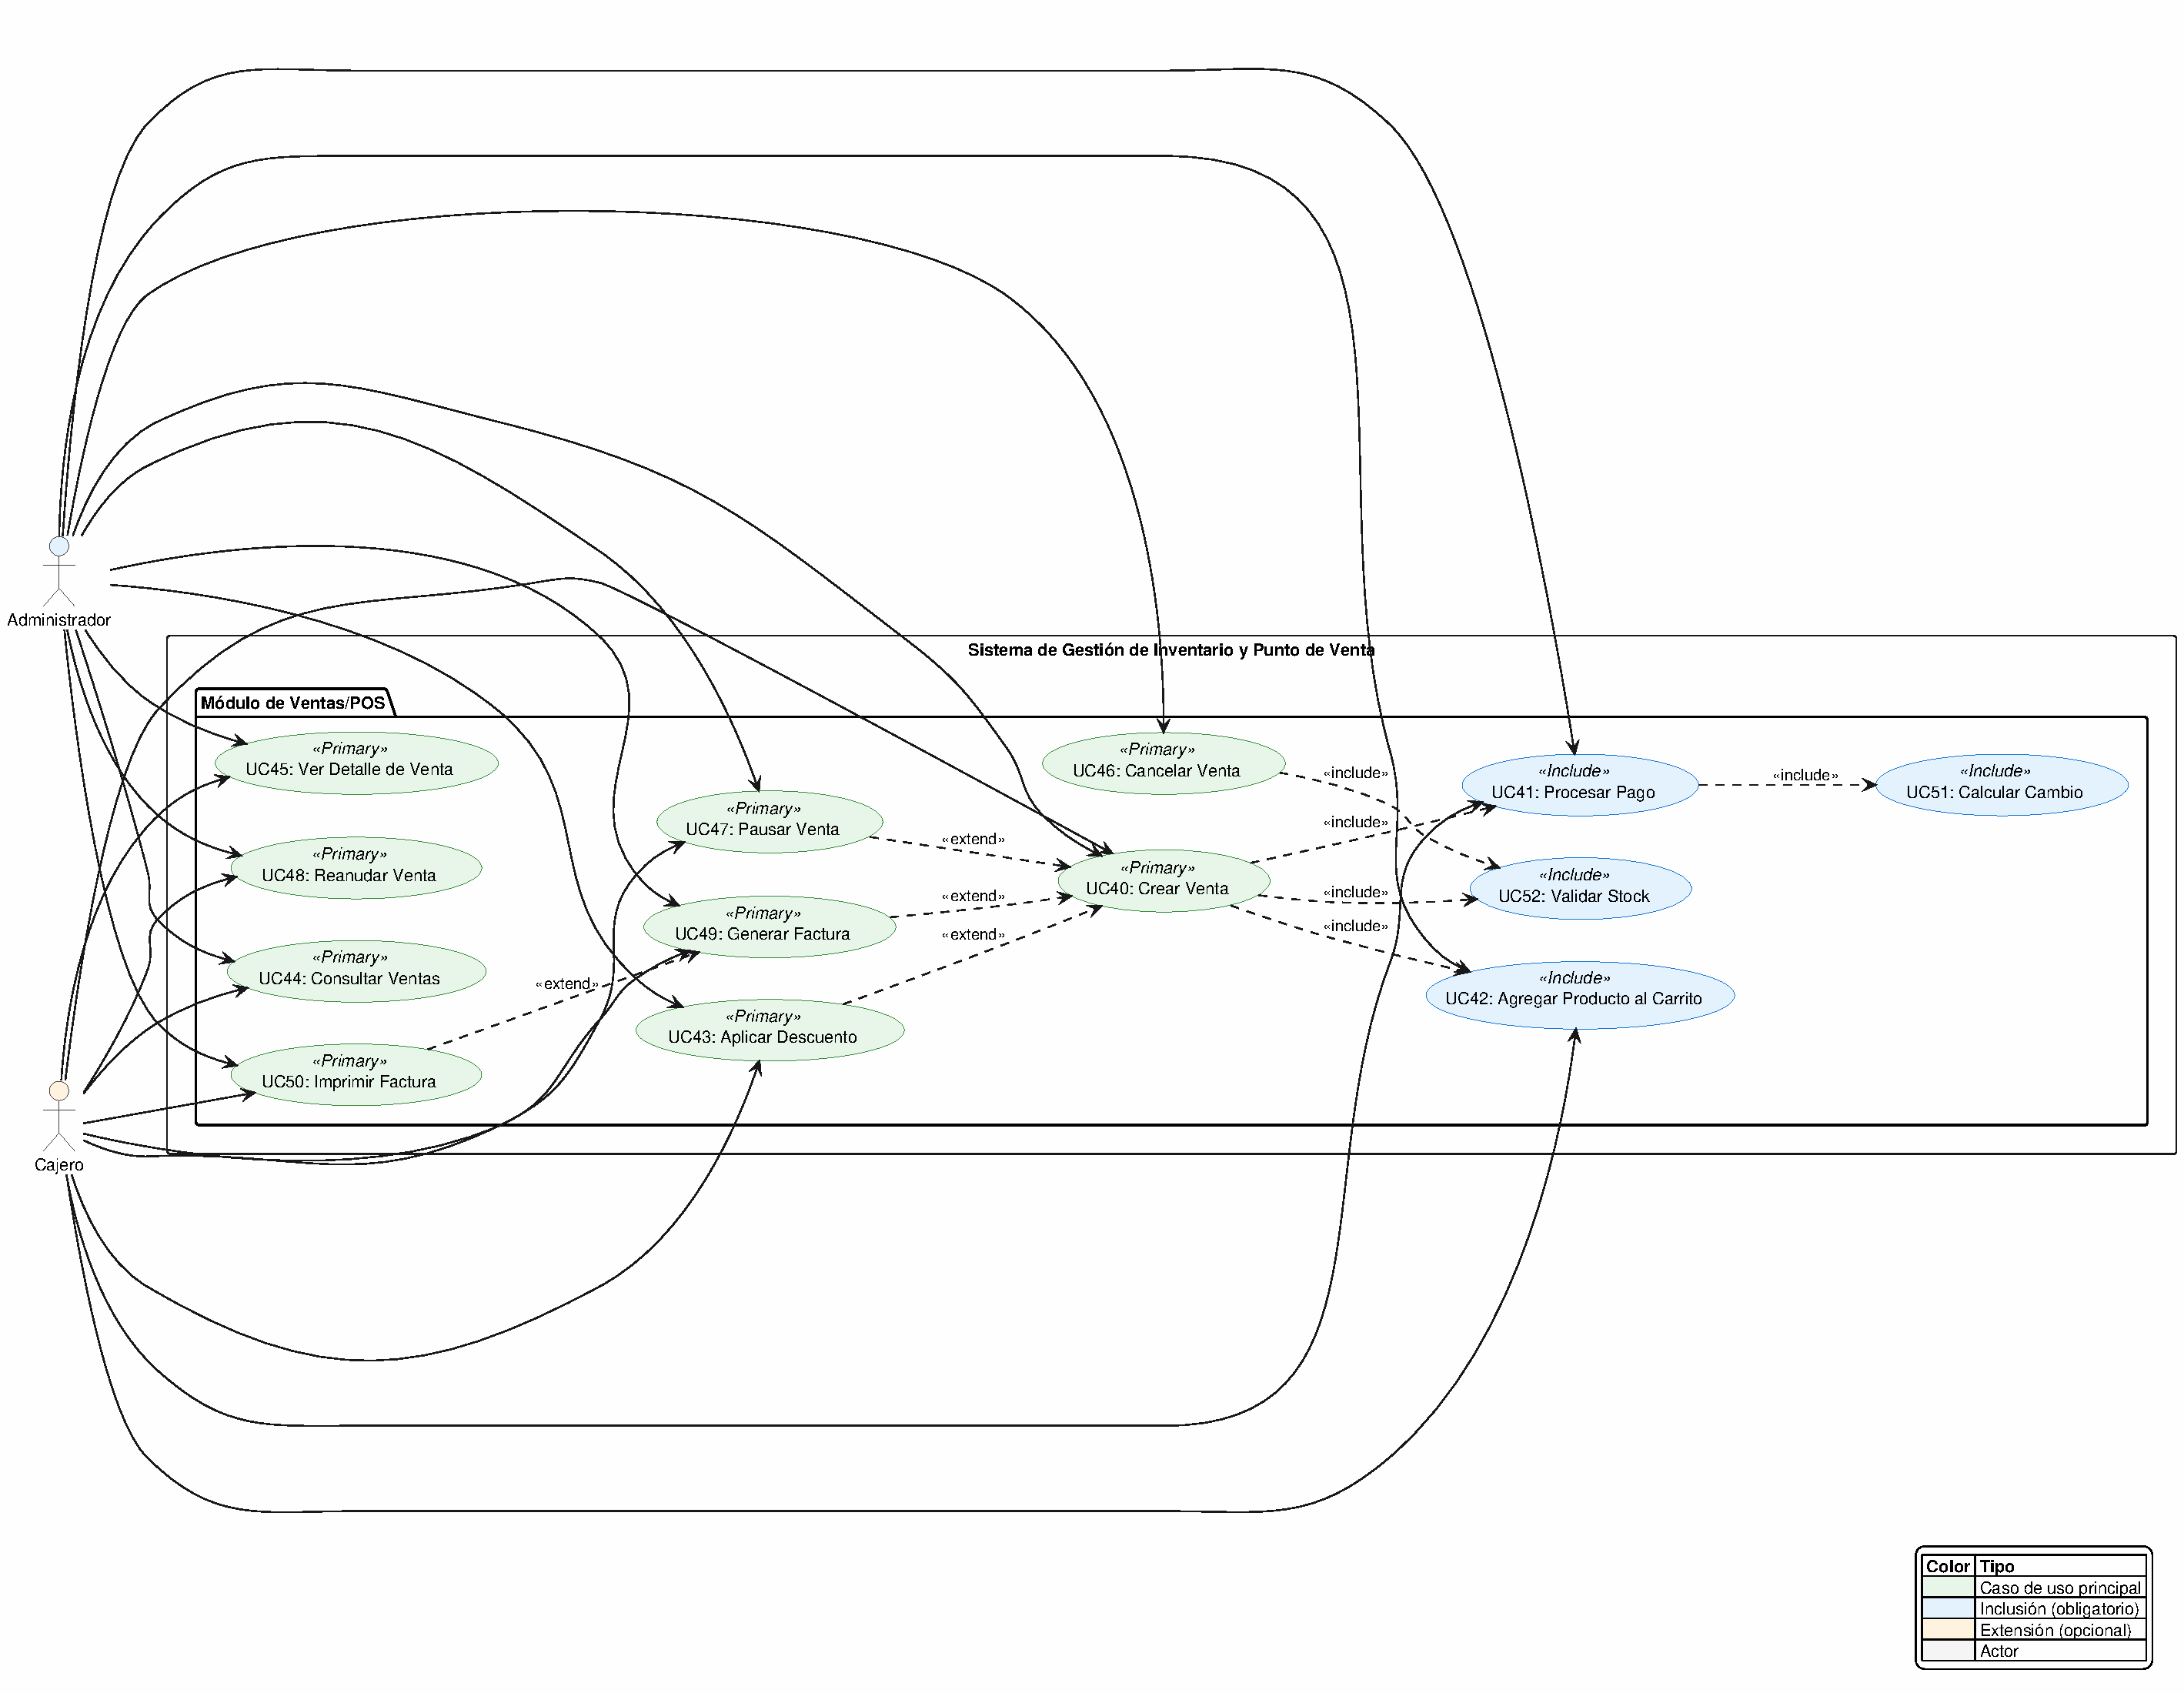
\includegraphics[width=0.9\textwidth]{Images/diagramas-uml/casos-de-uso/modulo-ventas}
	\caption{Diagrama de casos de uso - Módulo de ventas}
	\label{fig:cu-ventas}
\end{figure}

El módulo de clientes (Figura \ref{fig:cu-clientes}) permite gestionar la información de los clientes del negocio. Todos los roles pueden consultar clientes, mientras que los administradores y cajeros pueden registrar nuevos clientes y actualizar su información. Los administradores también pueden eliminar clientes (soft delete).

\begin{figure}[H]
	\centering
	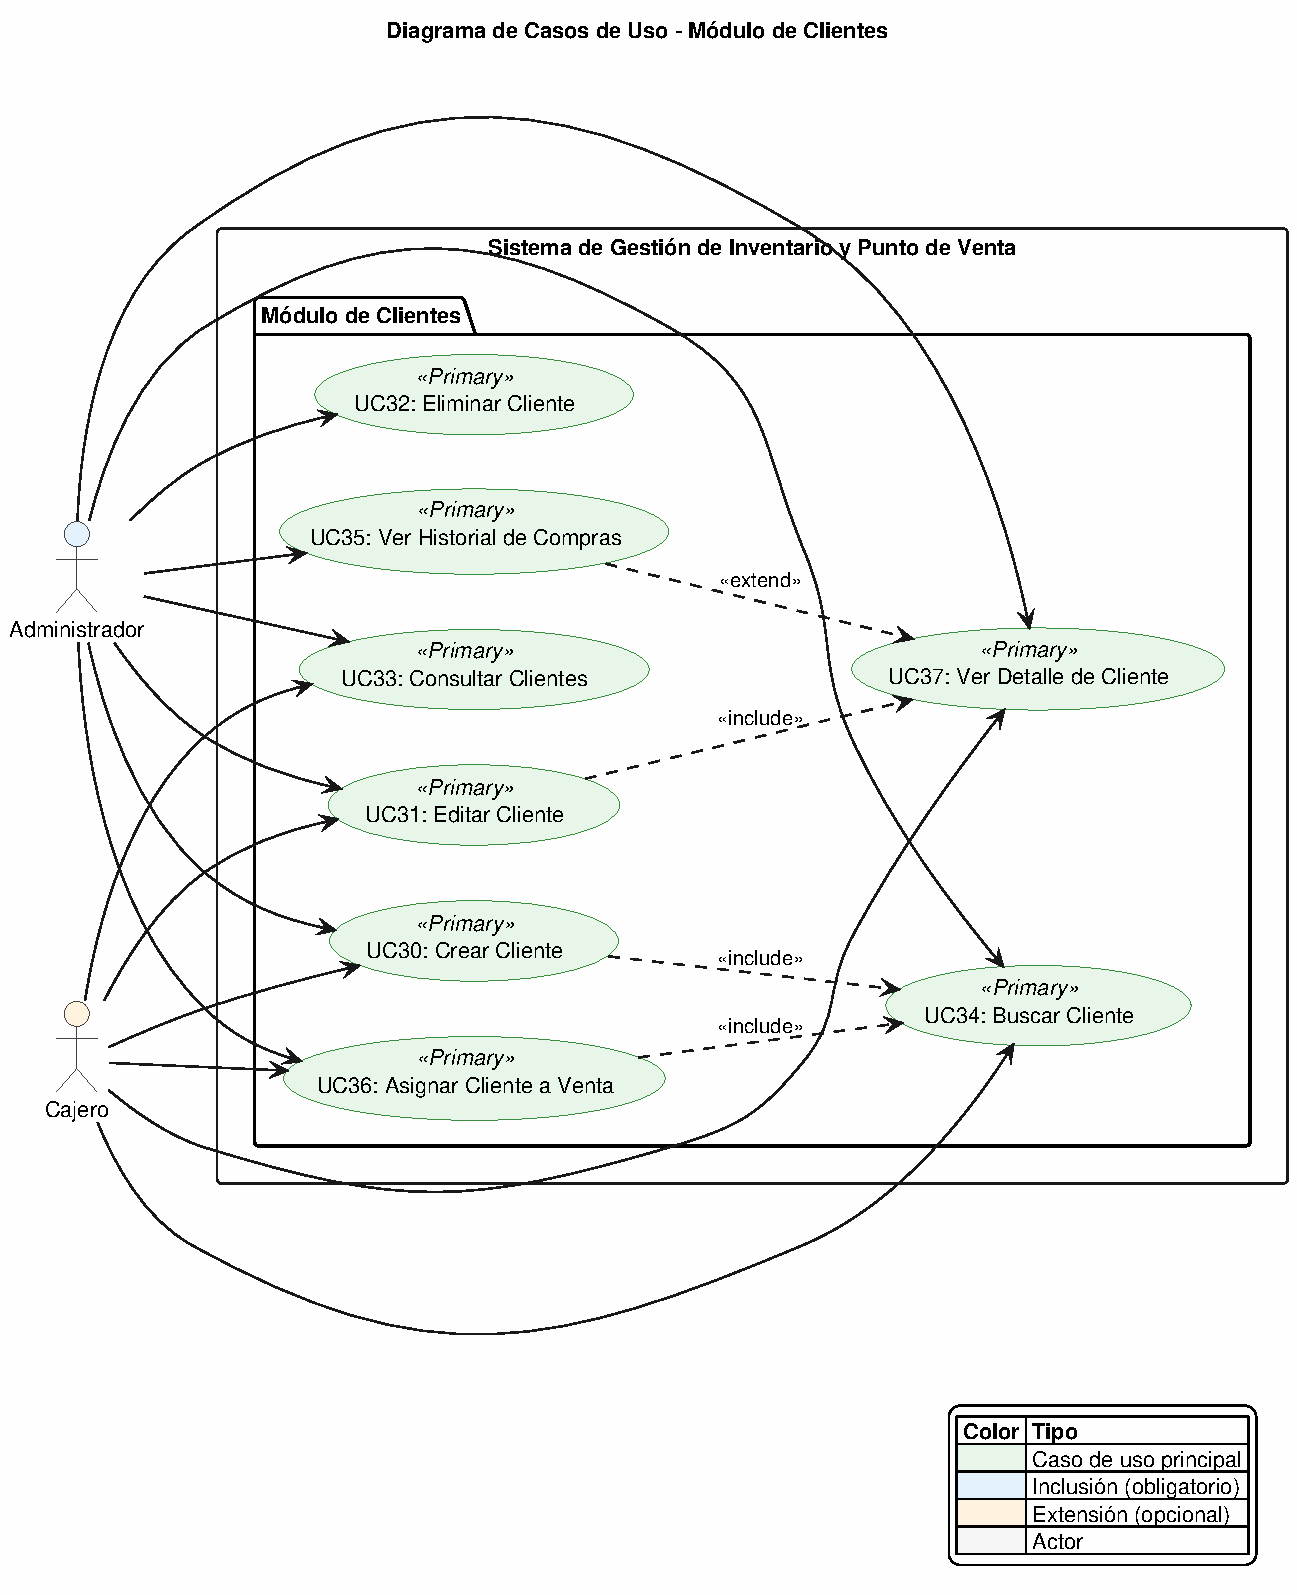
\includegraphics[width=0.9\textwidth]{Images/diagramas-uml/casos-de-uso/modulo-clientes}
	\caption{Diagrama de casos de uso - Módulo de clientes}
	\label{fig:cu-clientes}
\end{figure}

El módulo de reportes (Figura \ref{fig:cu-reportes}) proporciona acceso a métricas y estadísticas del negocio. Los administradores y cajeros pueden acceder al dashboard con KPIs en tiempo real, reportes de ventas, productos más vendidos, y tendencias. Los administradores también pueden exportar reportes en diferentes formatos.

\begin{figure}[H]
	\centering
	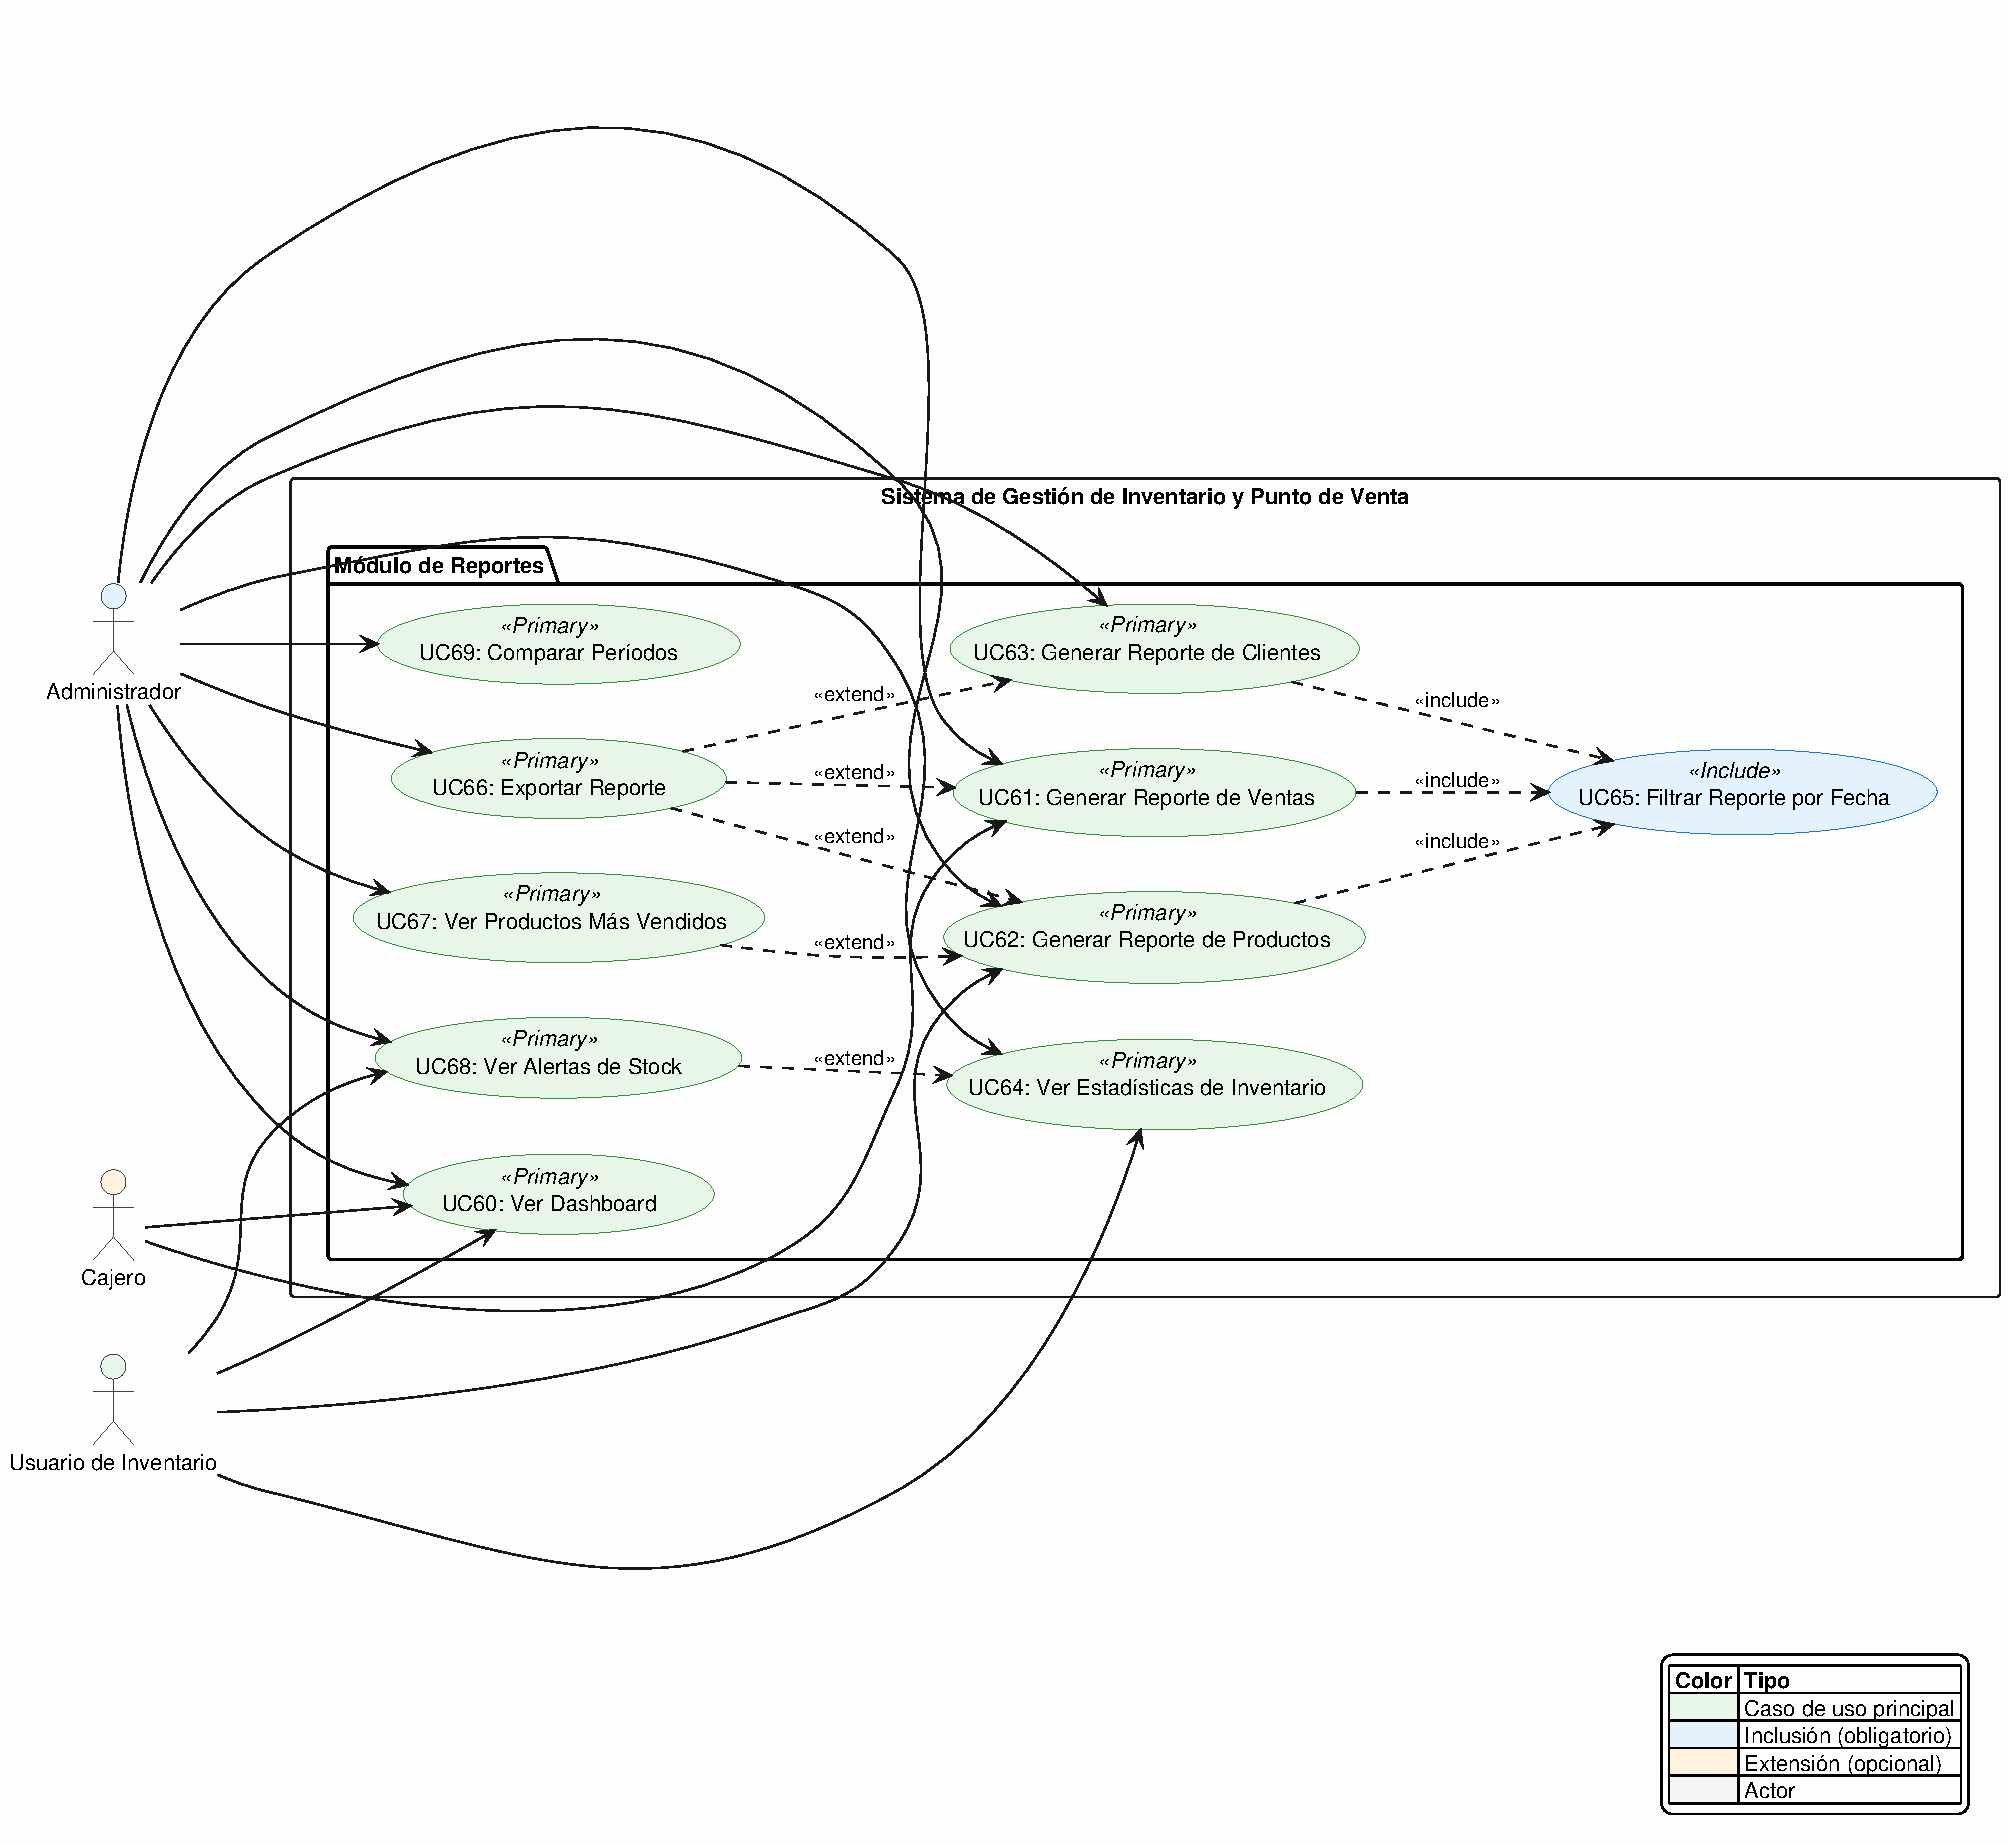
\includegraphics[width=0.9\textwidth]{Images/diagramas-uml/casos-de-uso/modulo-reportes}
	\caption{Diagrama de casos de uso - Módulo de reportes}
	\label{fig:cu-reportes}
\end{figure}

El módulo de configuración (Figura \ref{fig:cu-configuracion}) permite a los administradores gestionar usuarios del sistema, asignar roles, configurar parámetros del negocio, y ajustar configuraciones generales.

\begin{figure}[H]
	\centering
	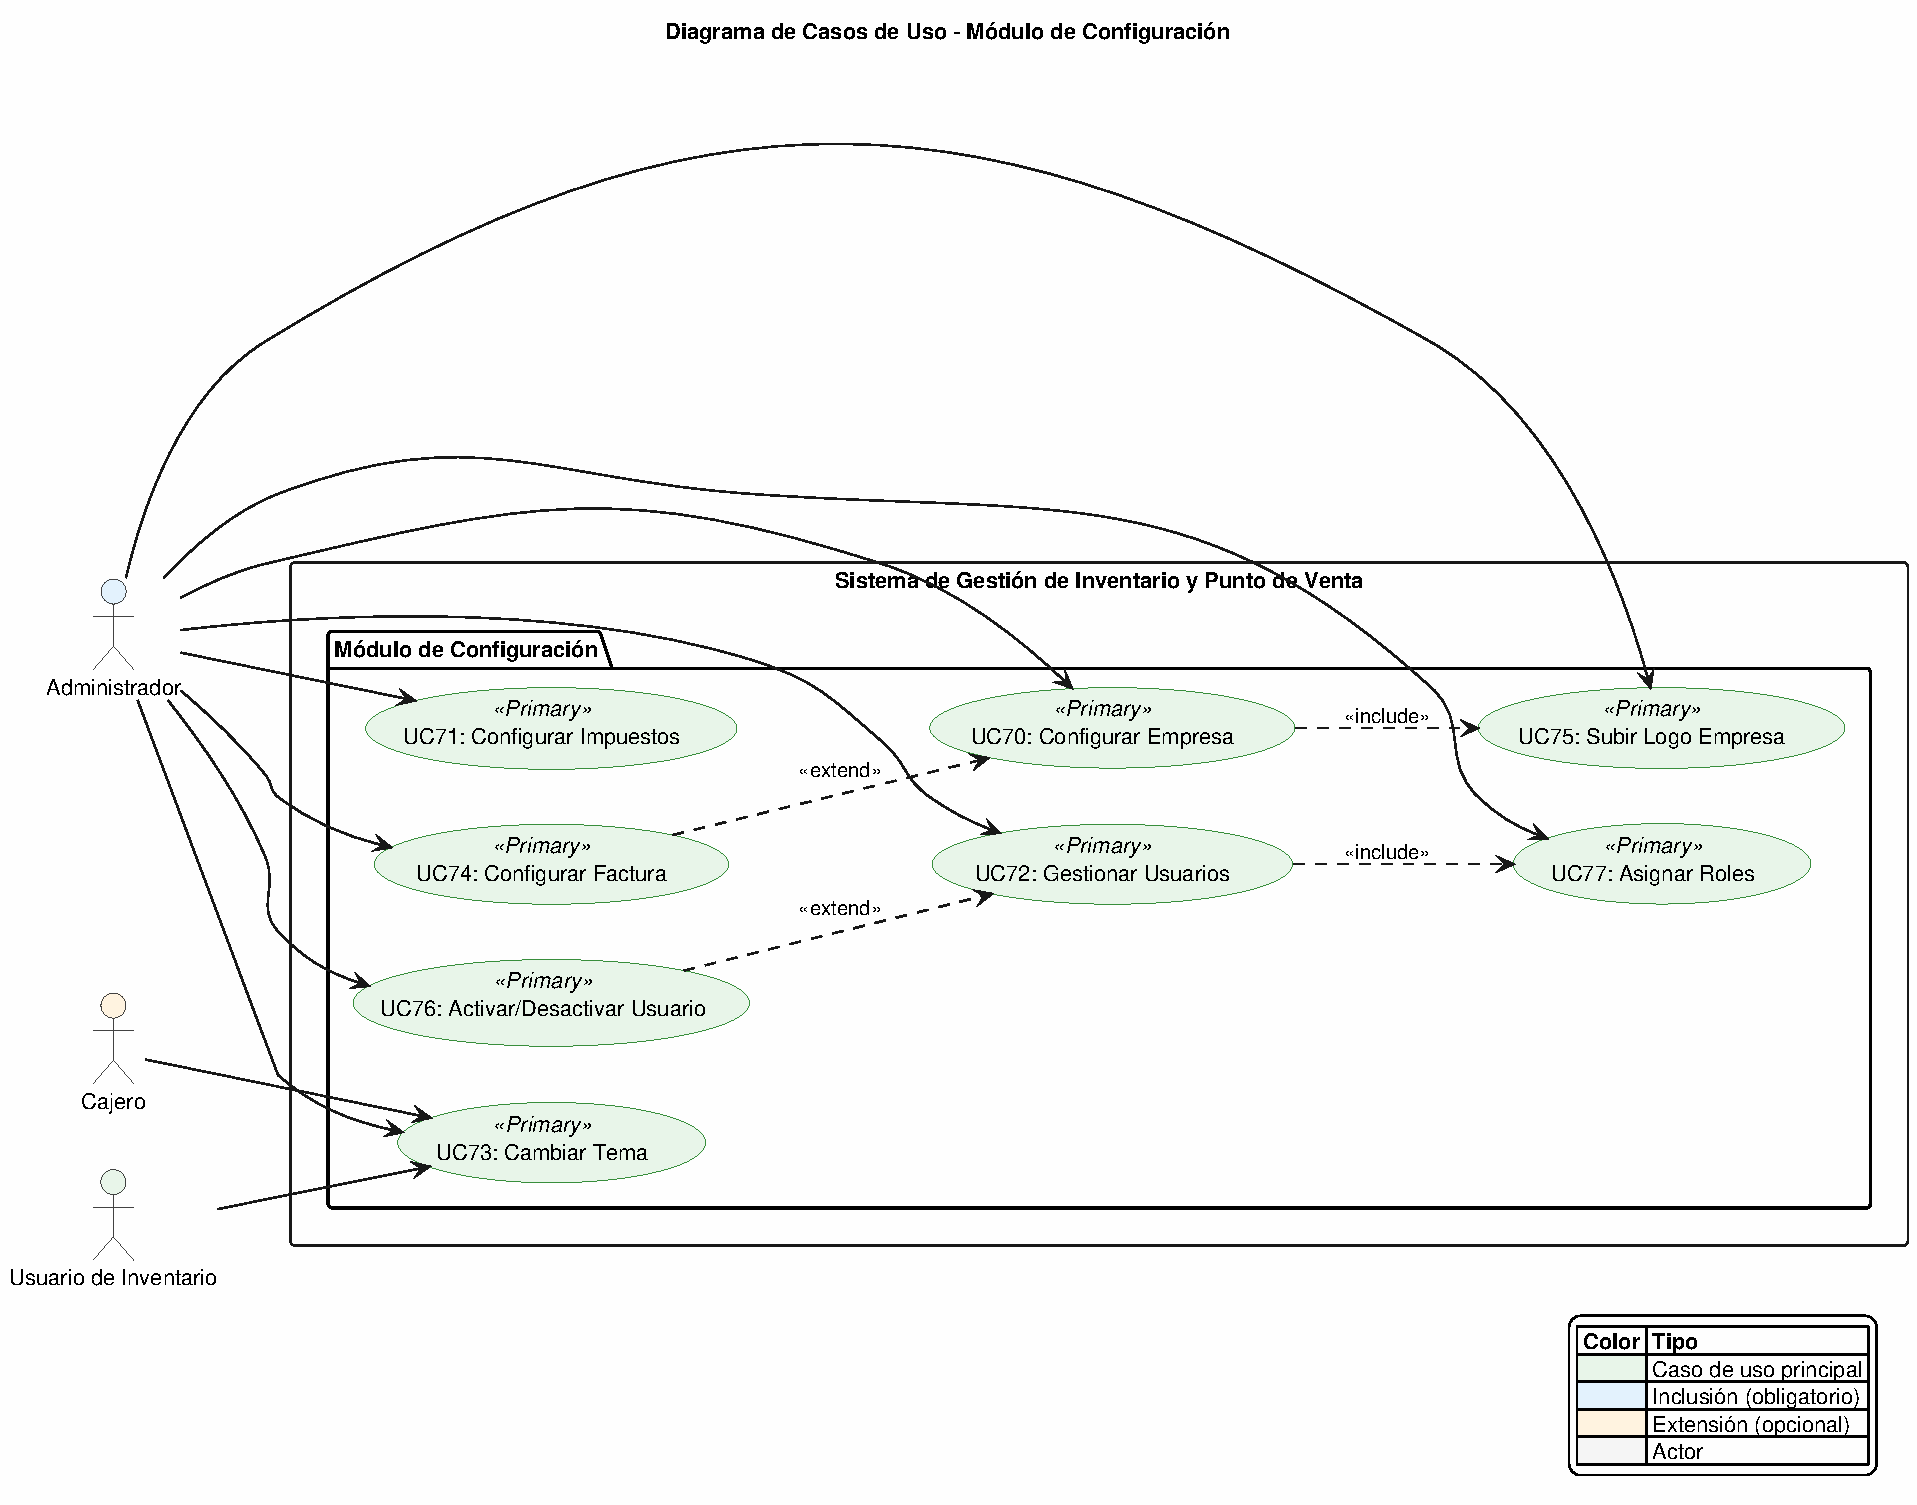
\includegraphics[width=0.9\textwidth]{Images/diagramas-uml/casos-de-uso/modulo-configuracion}
	\caption{Diagrama de casos de uso - Módulo de configuración}
	\label{fig:cu-configuracion}
\end{figure}

El módulo de categorías (Figura \ref{fig:cu-categorias}) permite organizar los productos en categorías jerárquicas, facilitando la búsqueda y gestión del inventario. Los administradores y usuarios de inventario pueden crear, editar, eliminar y consultar categorías.

\begin{figure}[H]
	\centering
	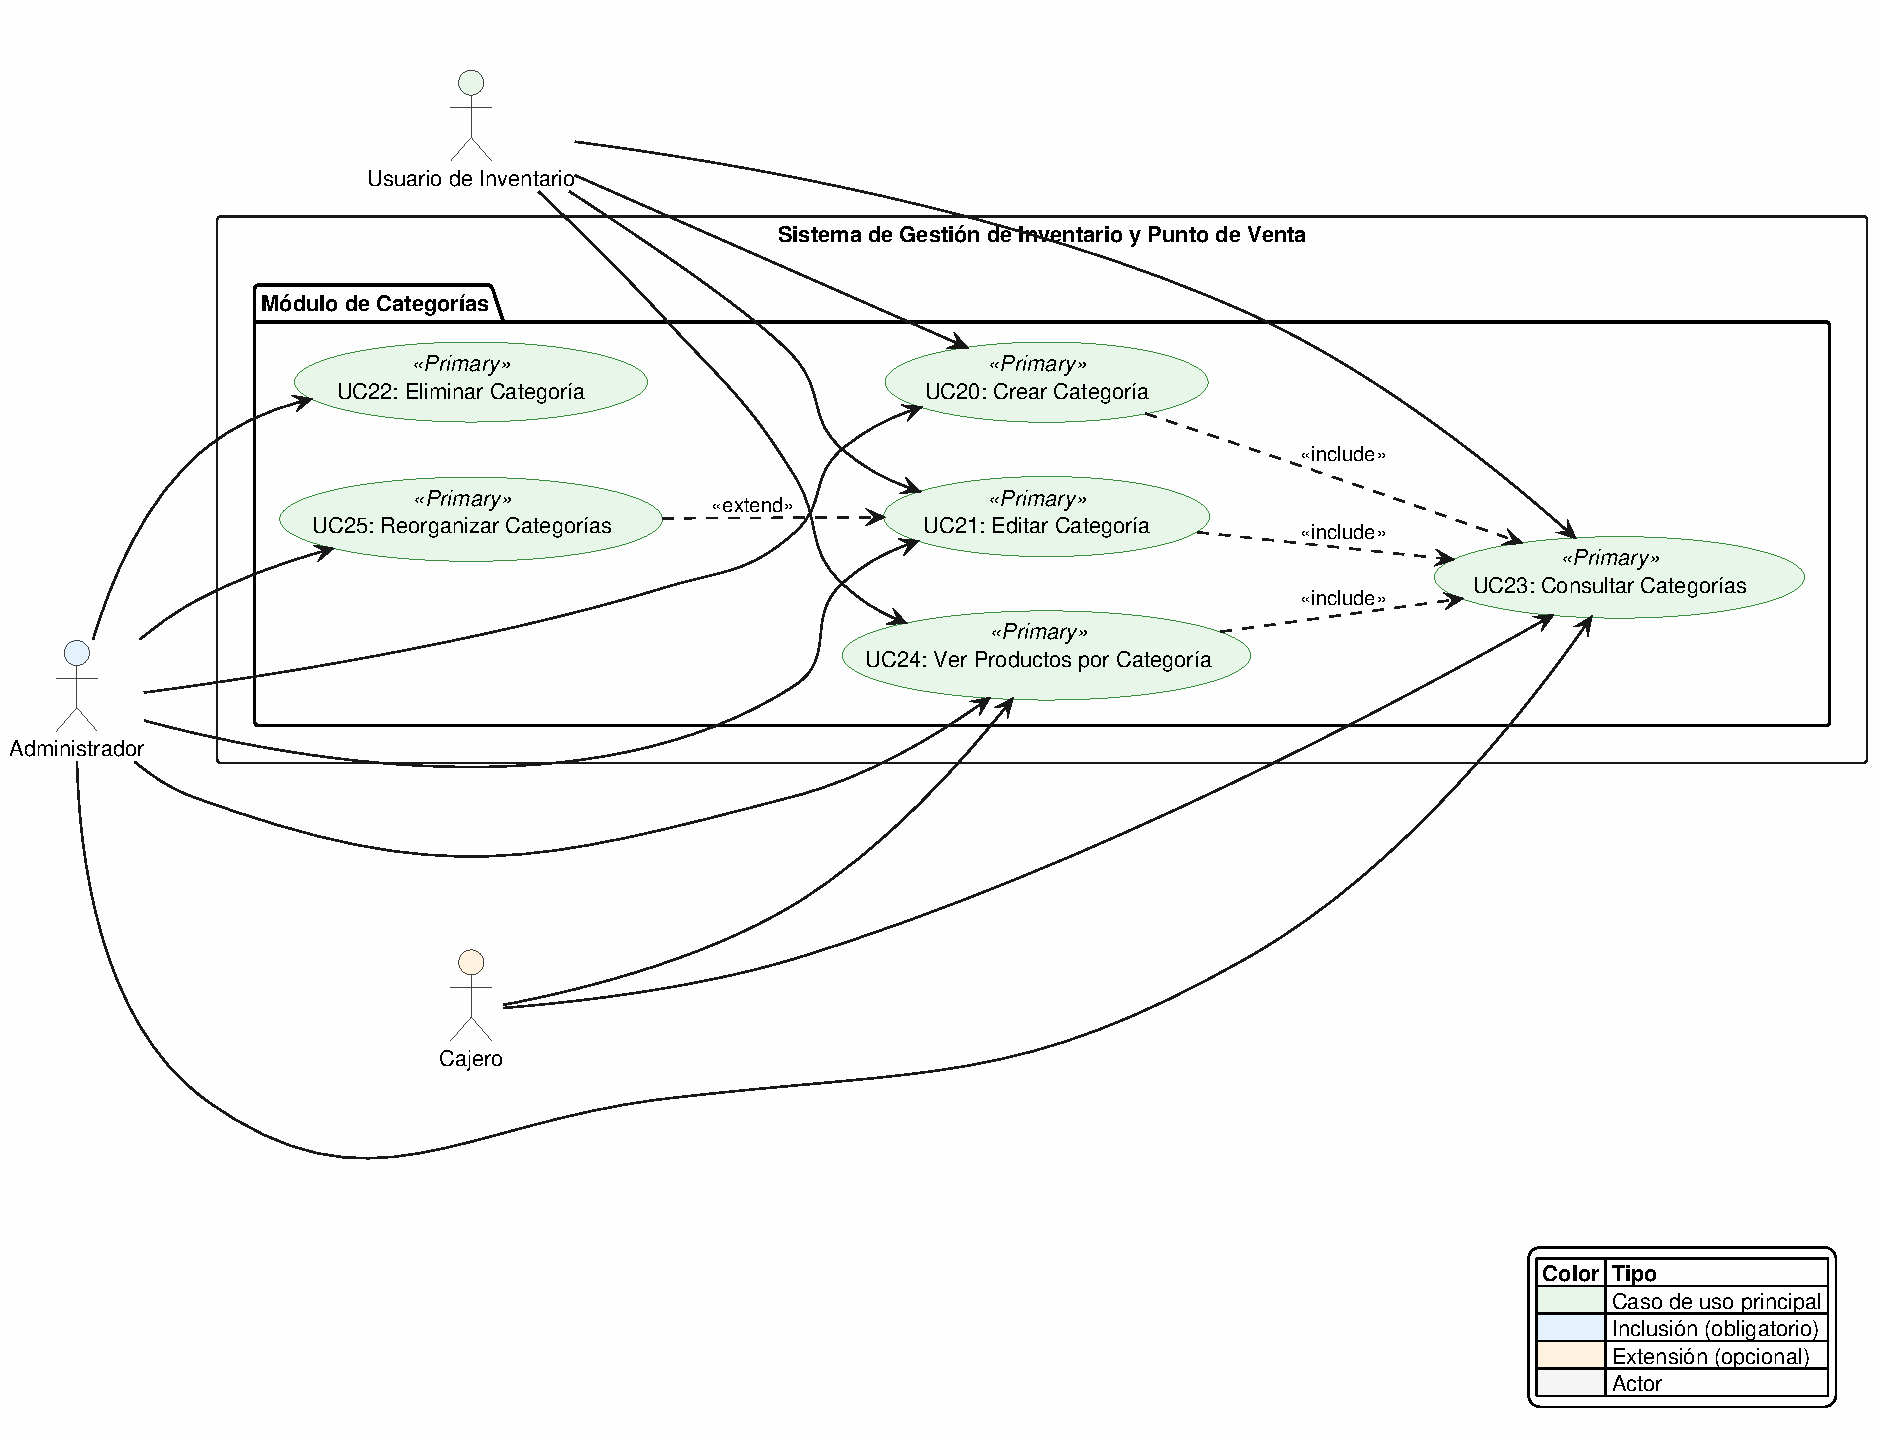
\includegraphics[width=0.9\textwidth]{Images/diagramas-uml/casos-de-uso/modulo-categorias}
	\caption{Diagrama de casos de uso - Módulo de categorías}
	\label{fig:cu-categorias}
\end{figure}

\subsection{Diagramas de componentes}

Los diagramas de componentes describen la arquitectura técnica interna del sistema, mostrando cómo se organizan los módulos del backend implementado con NestJS y cómo interactúan entre sí y con las dependencias externas.

El módulo de autenticación (Figura \ref{fig:comp-auth}) implementa la seguridad del sistema mediante JWT (JSON Web Tokens). El \texttt{AuthController} expone los endpoints REST, el \texttt{AuthService} contiene la lógica de negocio de validación de credenciales y generación de tokens, los guards (\texttt{JwtAuthGuard} y \texttt{RolesGuard}) protegen las rutas, y las estrategias (\texttt{JwtStrategy}) implementan la validación de tokens. Utiliza \texttt{PrismaService} para acceso a datos, \texttt{JwtService} para gestión de tokens, y \texttt{bcrypt} para encriptación de contraseñas.

\begin{figure}[H]
	\centering
	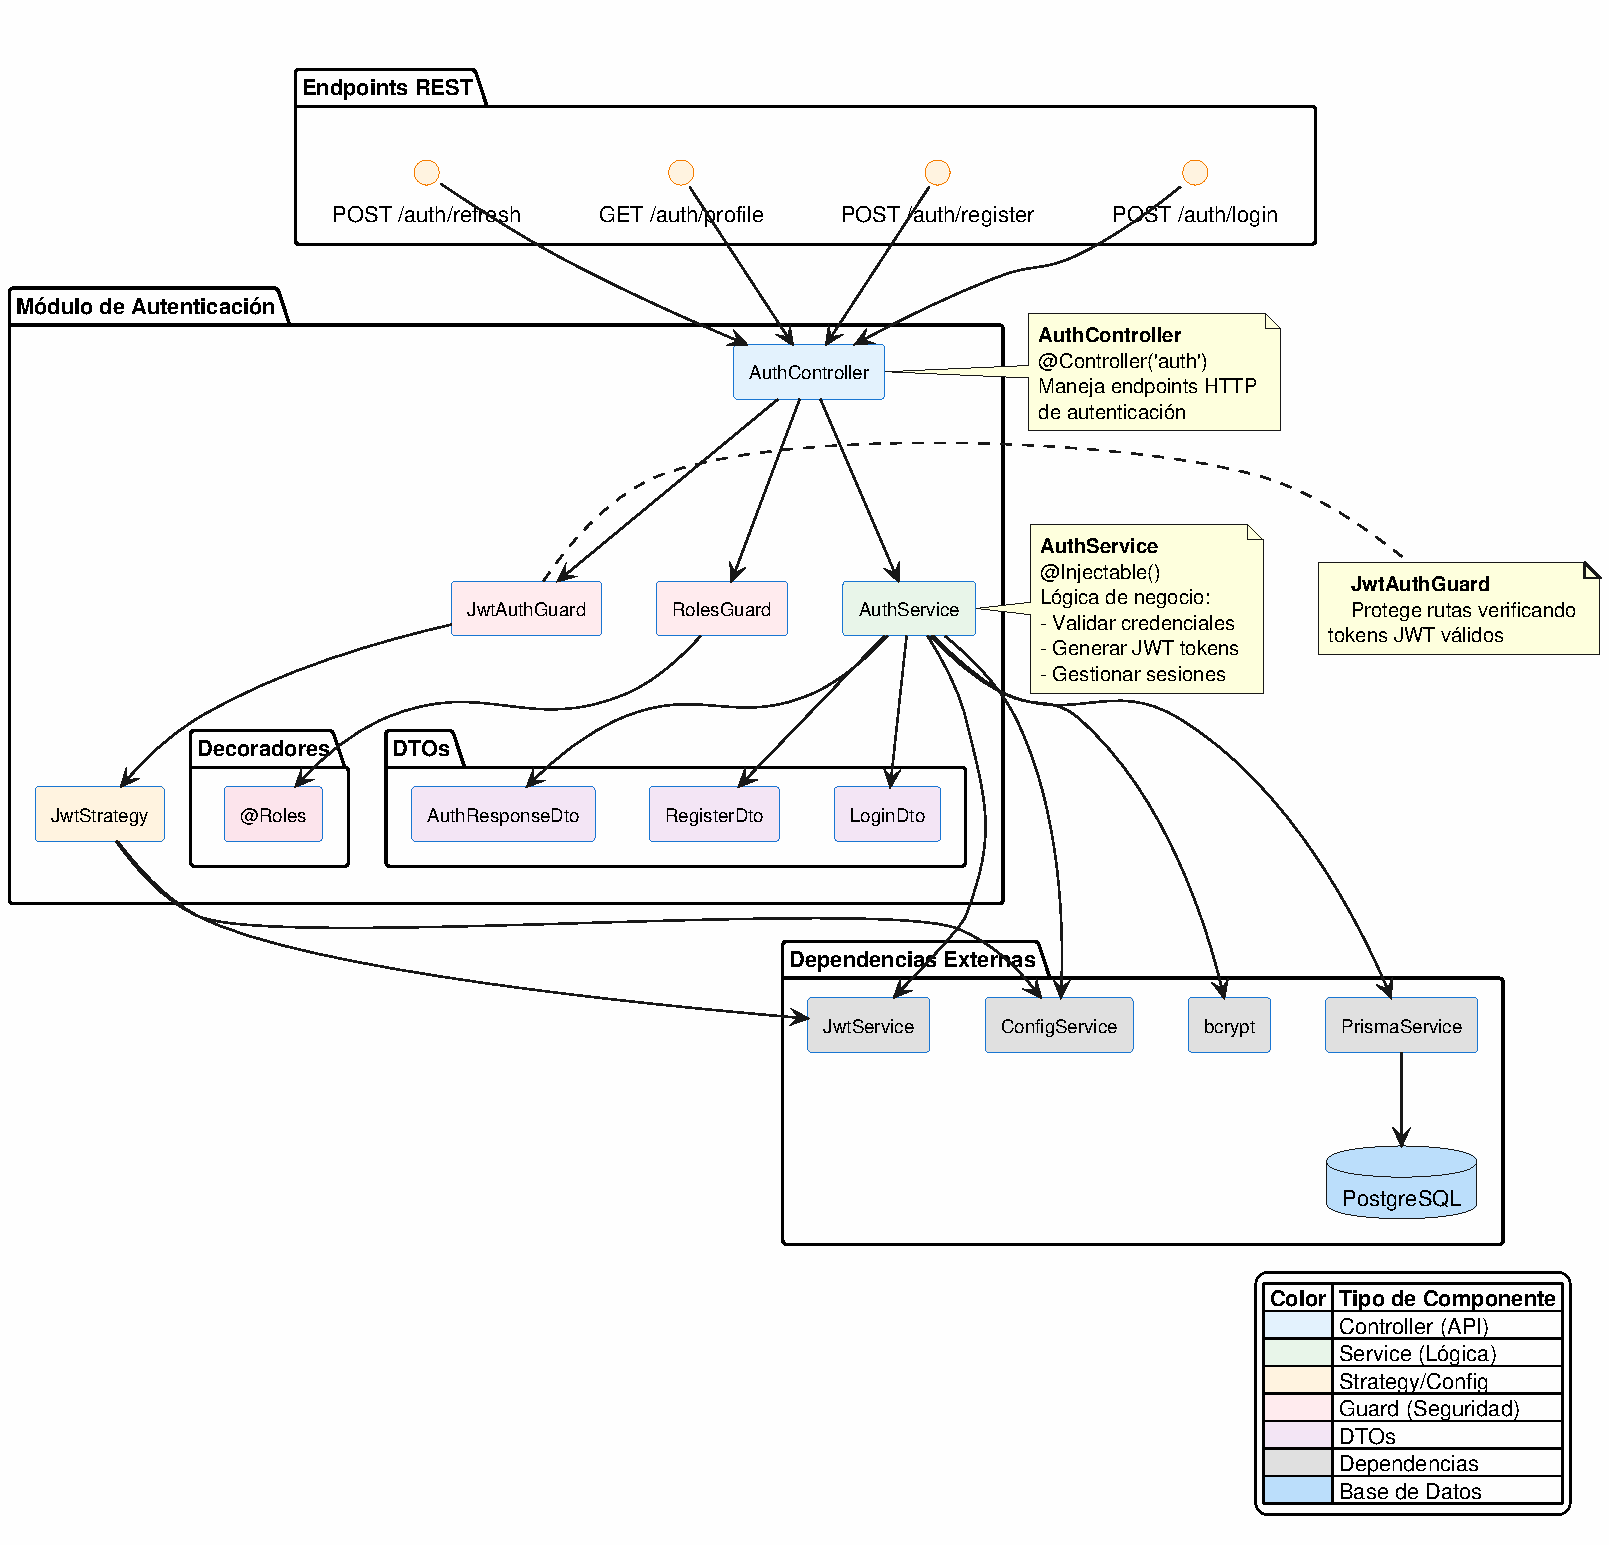
\includegraphics[width=0.85\textwidth]{Images/diagramas-uml/componentes/modulo-auth}
	\caption{Diagrama de componentes - Módulo de autenticación}
	\label{fig:comp-auth}
\end{figure}

El módulo de productos (Figura \ref{fig:comp-productos}) gestiona el inventario completo. El \texttt{ProductsController} expone endpoints para CRUD de productos, búsqueda y filtrado. El \texttt{ProductsService} implementa la lógica de negocio incluyendo control de stock, validaciones, y alertas. Se integra con \texttt{Cloudinary} para gestión de imágenes de productos y con \texttt{CategoriesService} para organización jerárquica.

\begin{figure}[H]
	\centering
	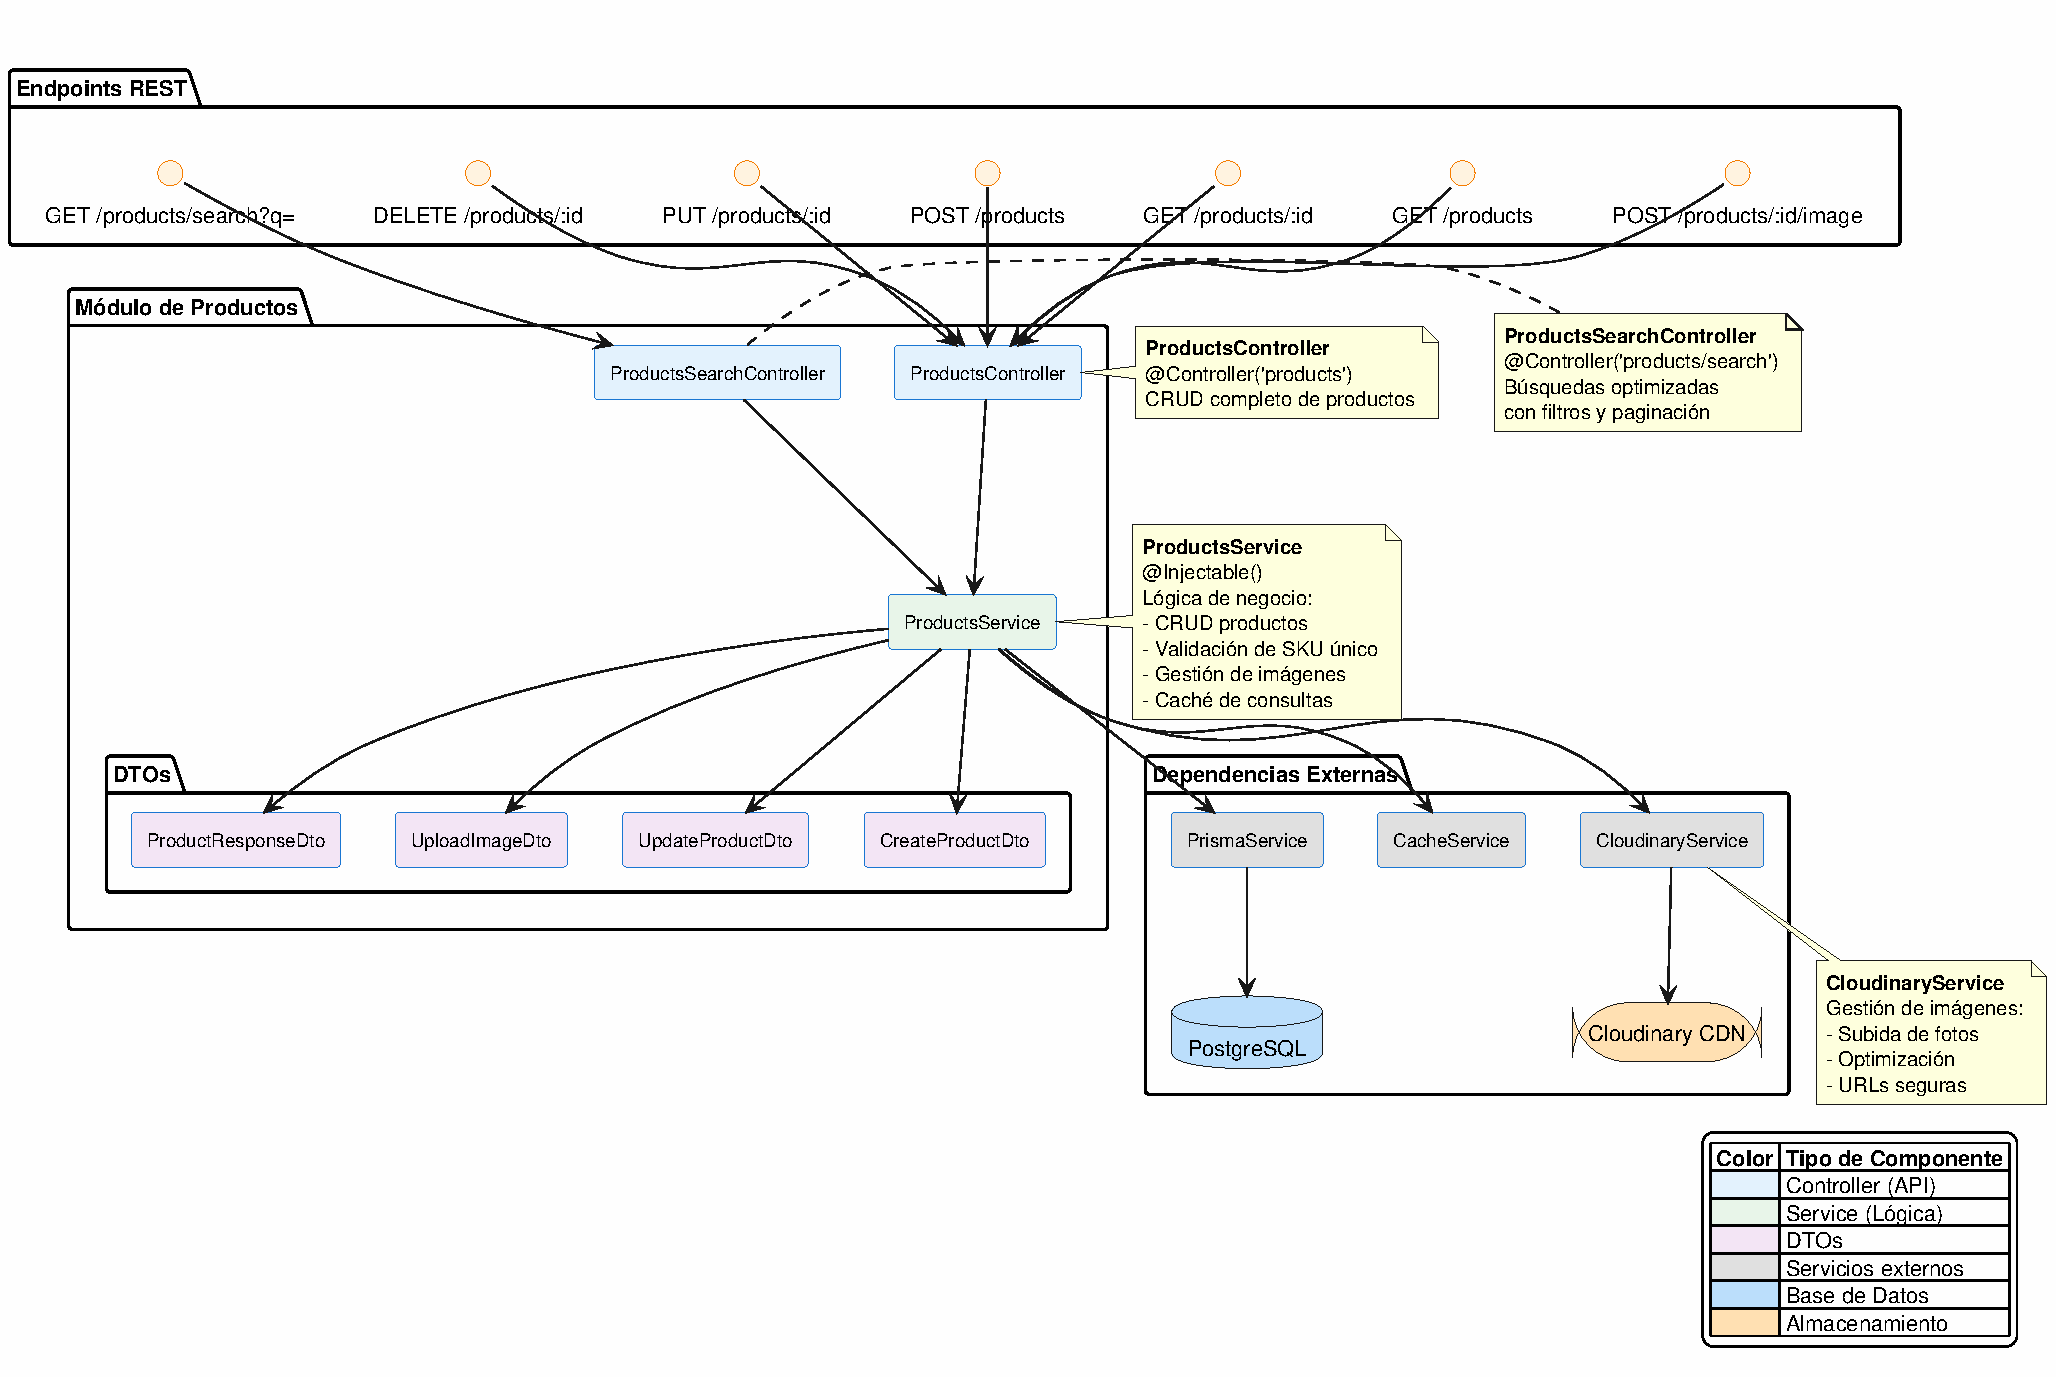
\includegraphics[width=0.85\textwidth]{Images/diagramas-uml/componentes/modulo-productos}
	\caption{Diagrama de componentes - Módulo de productos}
	\label{fig:comp-productos}
\end{figure}

El módulo de ventas (Figura \ref{fig:comp-ventas}) implementa el punto de venta con transacciones ACID. El \texttt{SalesController} expone endpoints para crear ventas, pausar/reanudar transacciones, y gestionar pagos. El \texttt{SalesService} implementa la lógica de negocio con transacciones atómicas que garantizan consistencia de datos. Se integra con \texttt{PrismaService} para persistencia y con servicios externos para generación de comprobantes.

\begin{figure}[H]
	\centering
	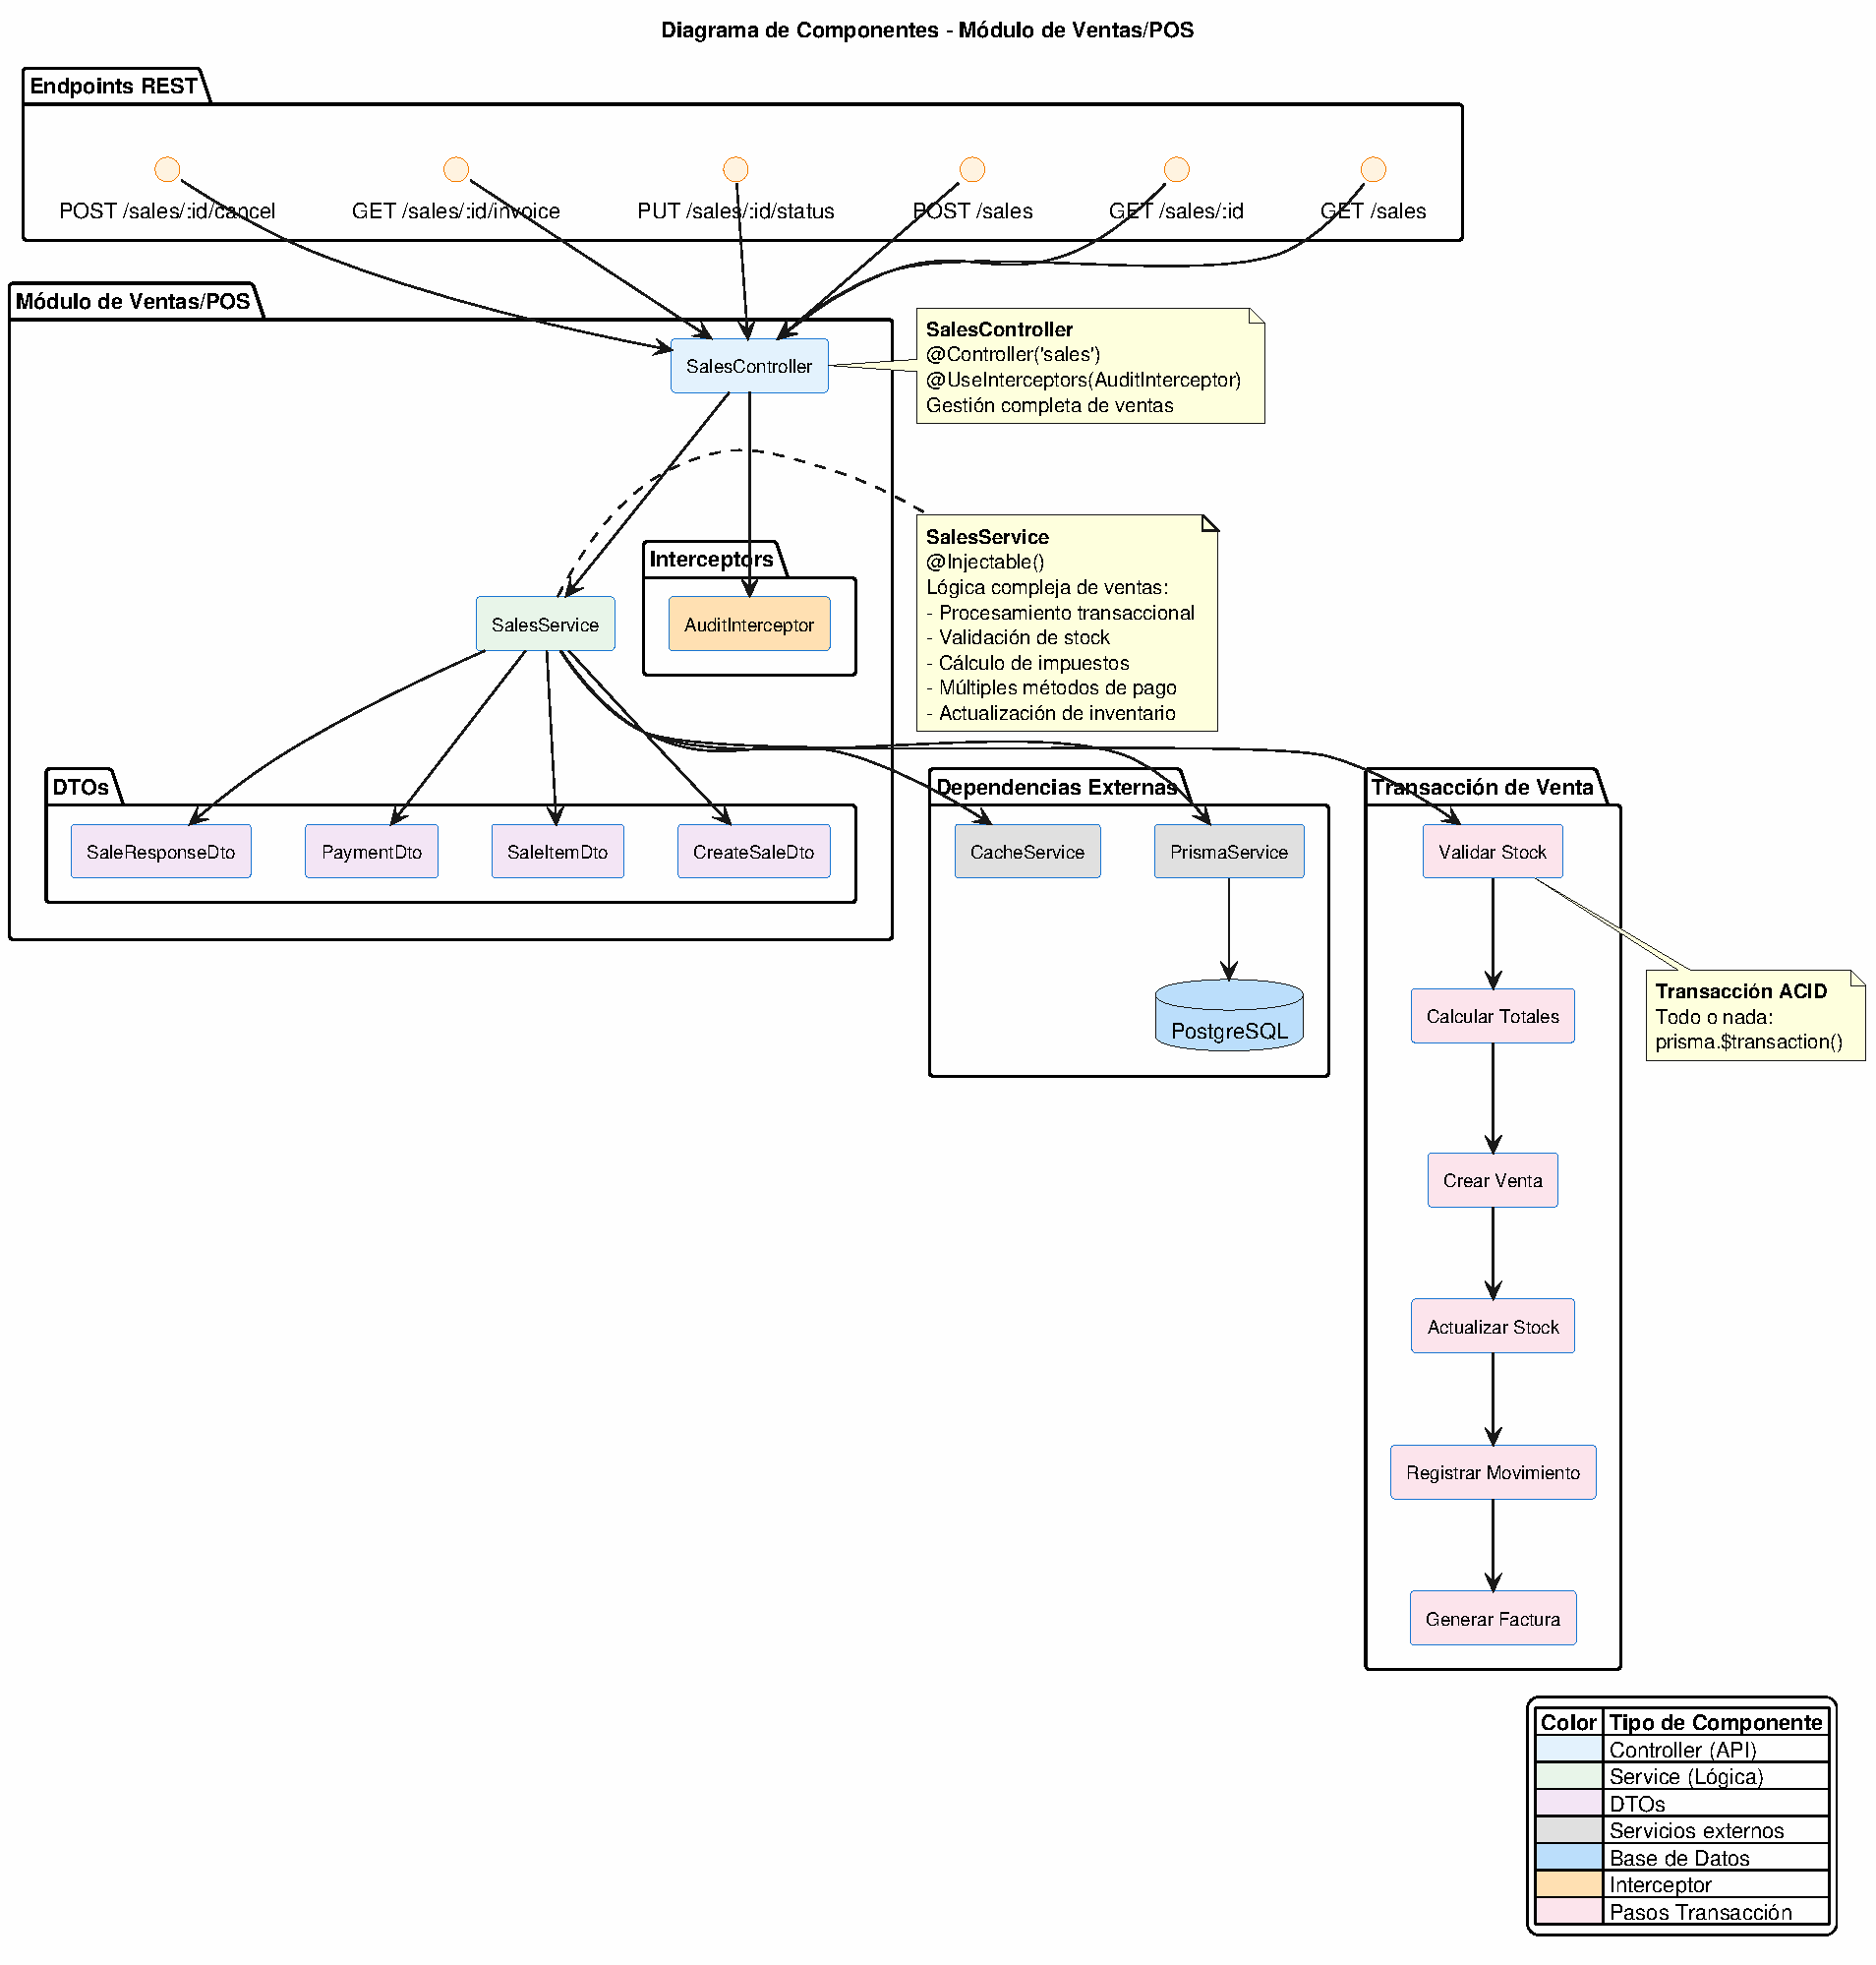
\includegraphics[width=0.85\textwidth]{Images/diagramas-uml/componentes/modulo-ventas}
	\caption{Diagrama de componentes - Módulo de ventas}
	\label{fig:comp-ventas}
\end{figure}

El módulo de clientes (Figura \ref{fig:comp-clientes}) permite gestionar la información de clientes. El \texttt{CustomersController} expone endpoints para CRUD de clientes, búsqueda y filtrado. El \texttt{CustomersService} implementa la lógica de negocio incluyendo historial de compras y soft delete para preservar integridad referencial con ventas históricas.

\begin{figure}[H]
	\centering
	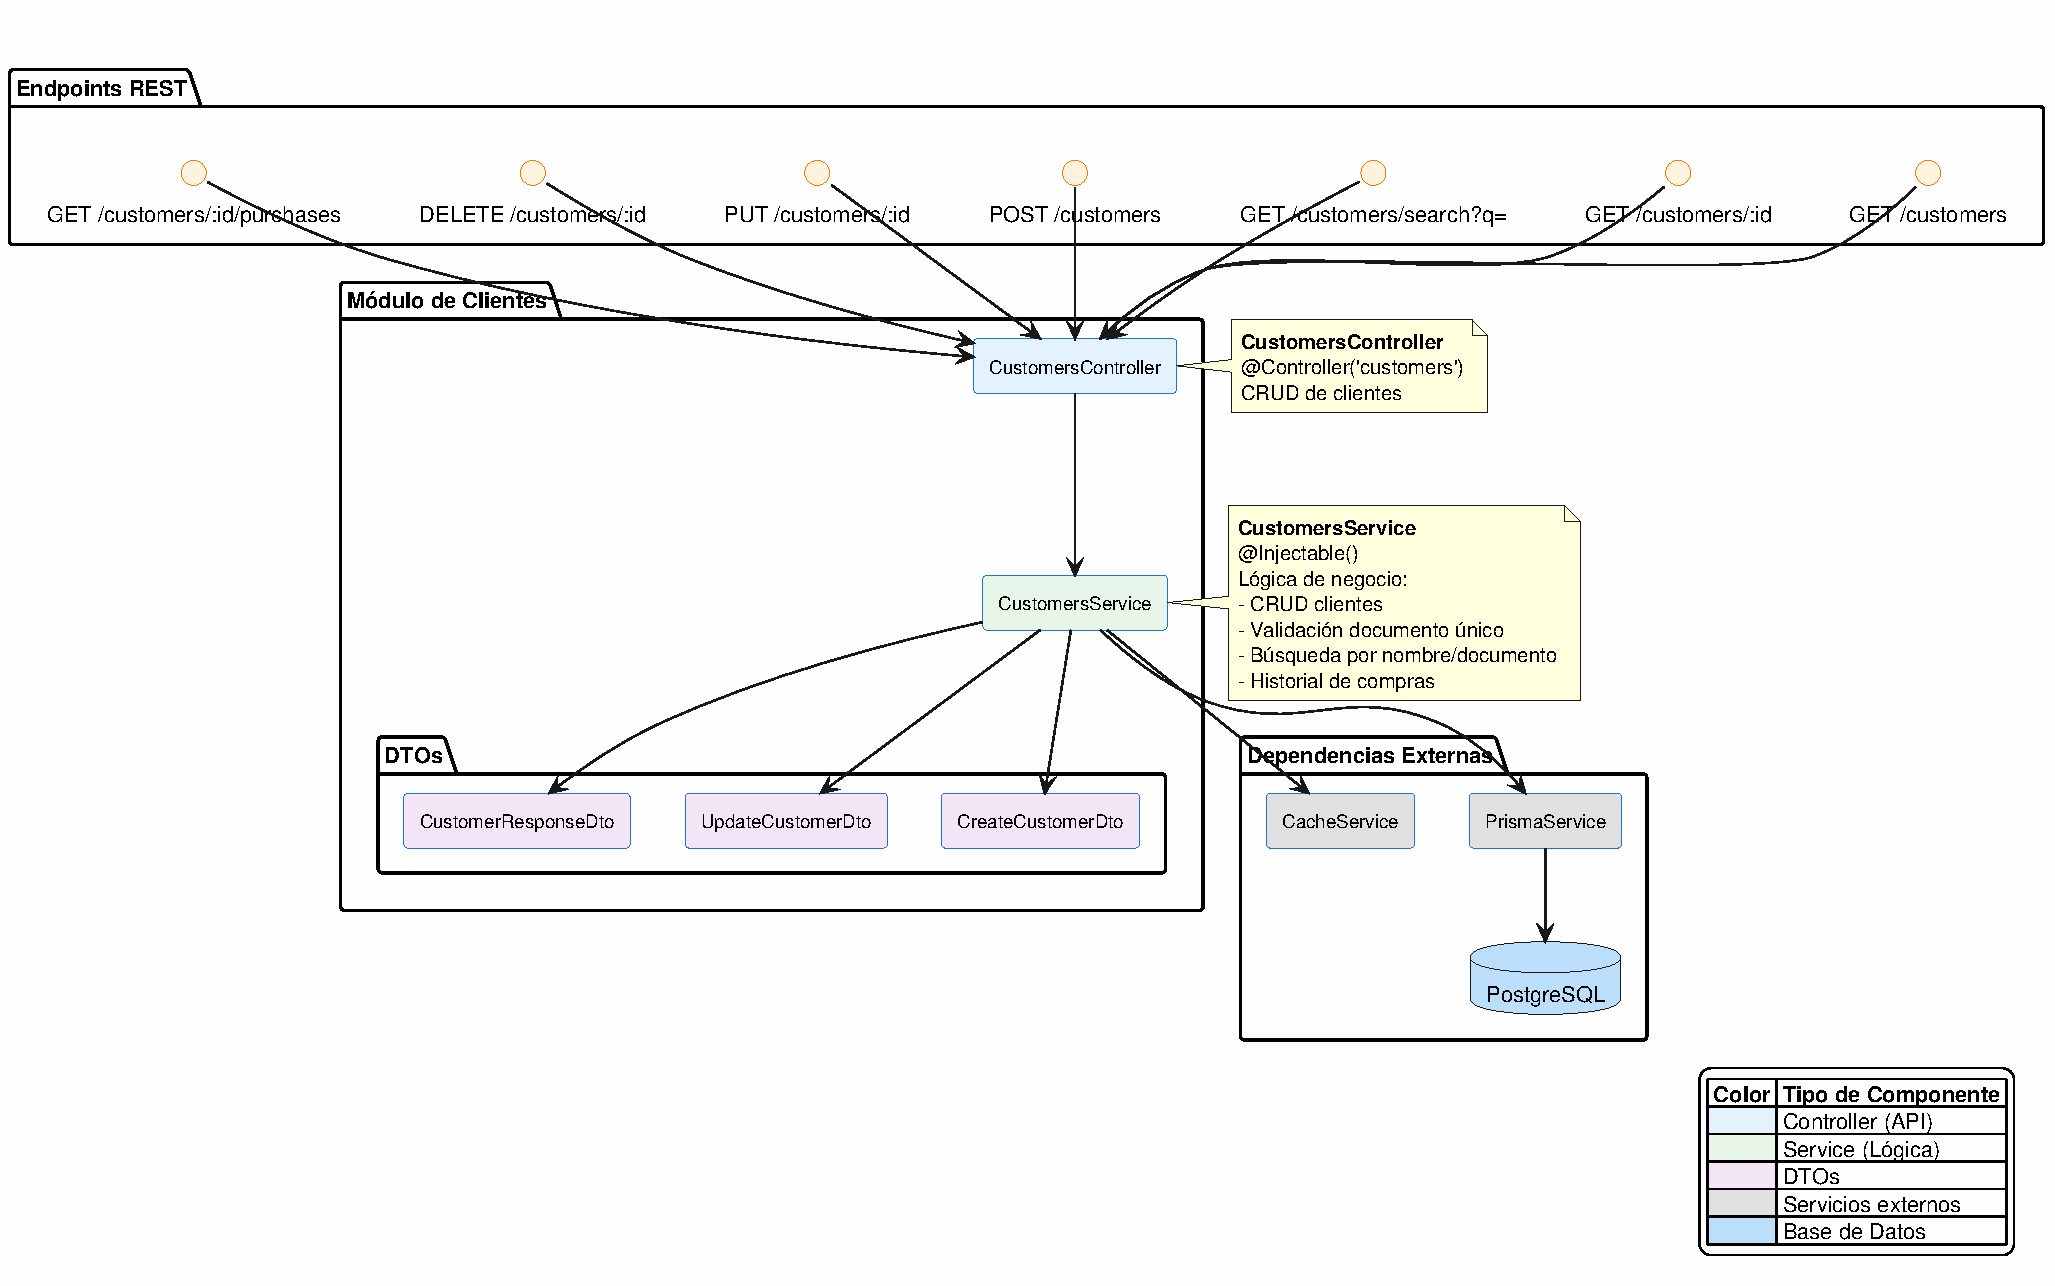
\includegraphics[width=0.85\textwidth]{Images/diagramas-uml/componentes/modulo-clientes}
	\caption{Diagrama de componentes - Módulo de clientes}
	\label{fig:comp-clientes}
\end{figure}

El módulo de reportes (Figura \ref{fig:comp-reportes}) genera métricas y estadísticas del negocio. El \texttt{ReportsController} expone endpoints para dashboards, reportes de ventas, productos más vendidos, y tendencias. El \texttt{ReportsService} implementa la lógica de negocio con consultas optimizadas y caché para mejorar rendimiento. Se integra con \texttt{ExportsService} para generación de reportes en PDF, Excel y CSV.

\begin{figure}[H]
	\centering
	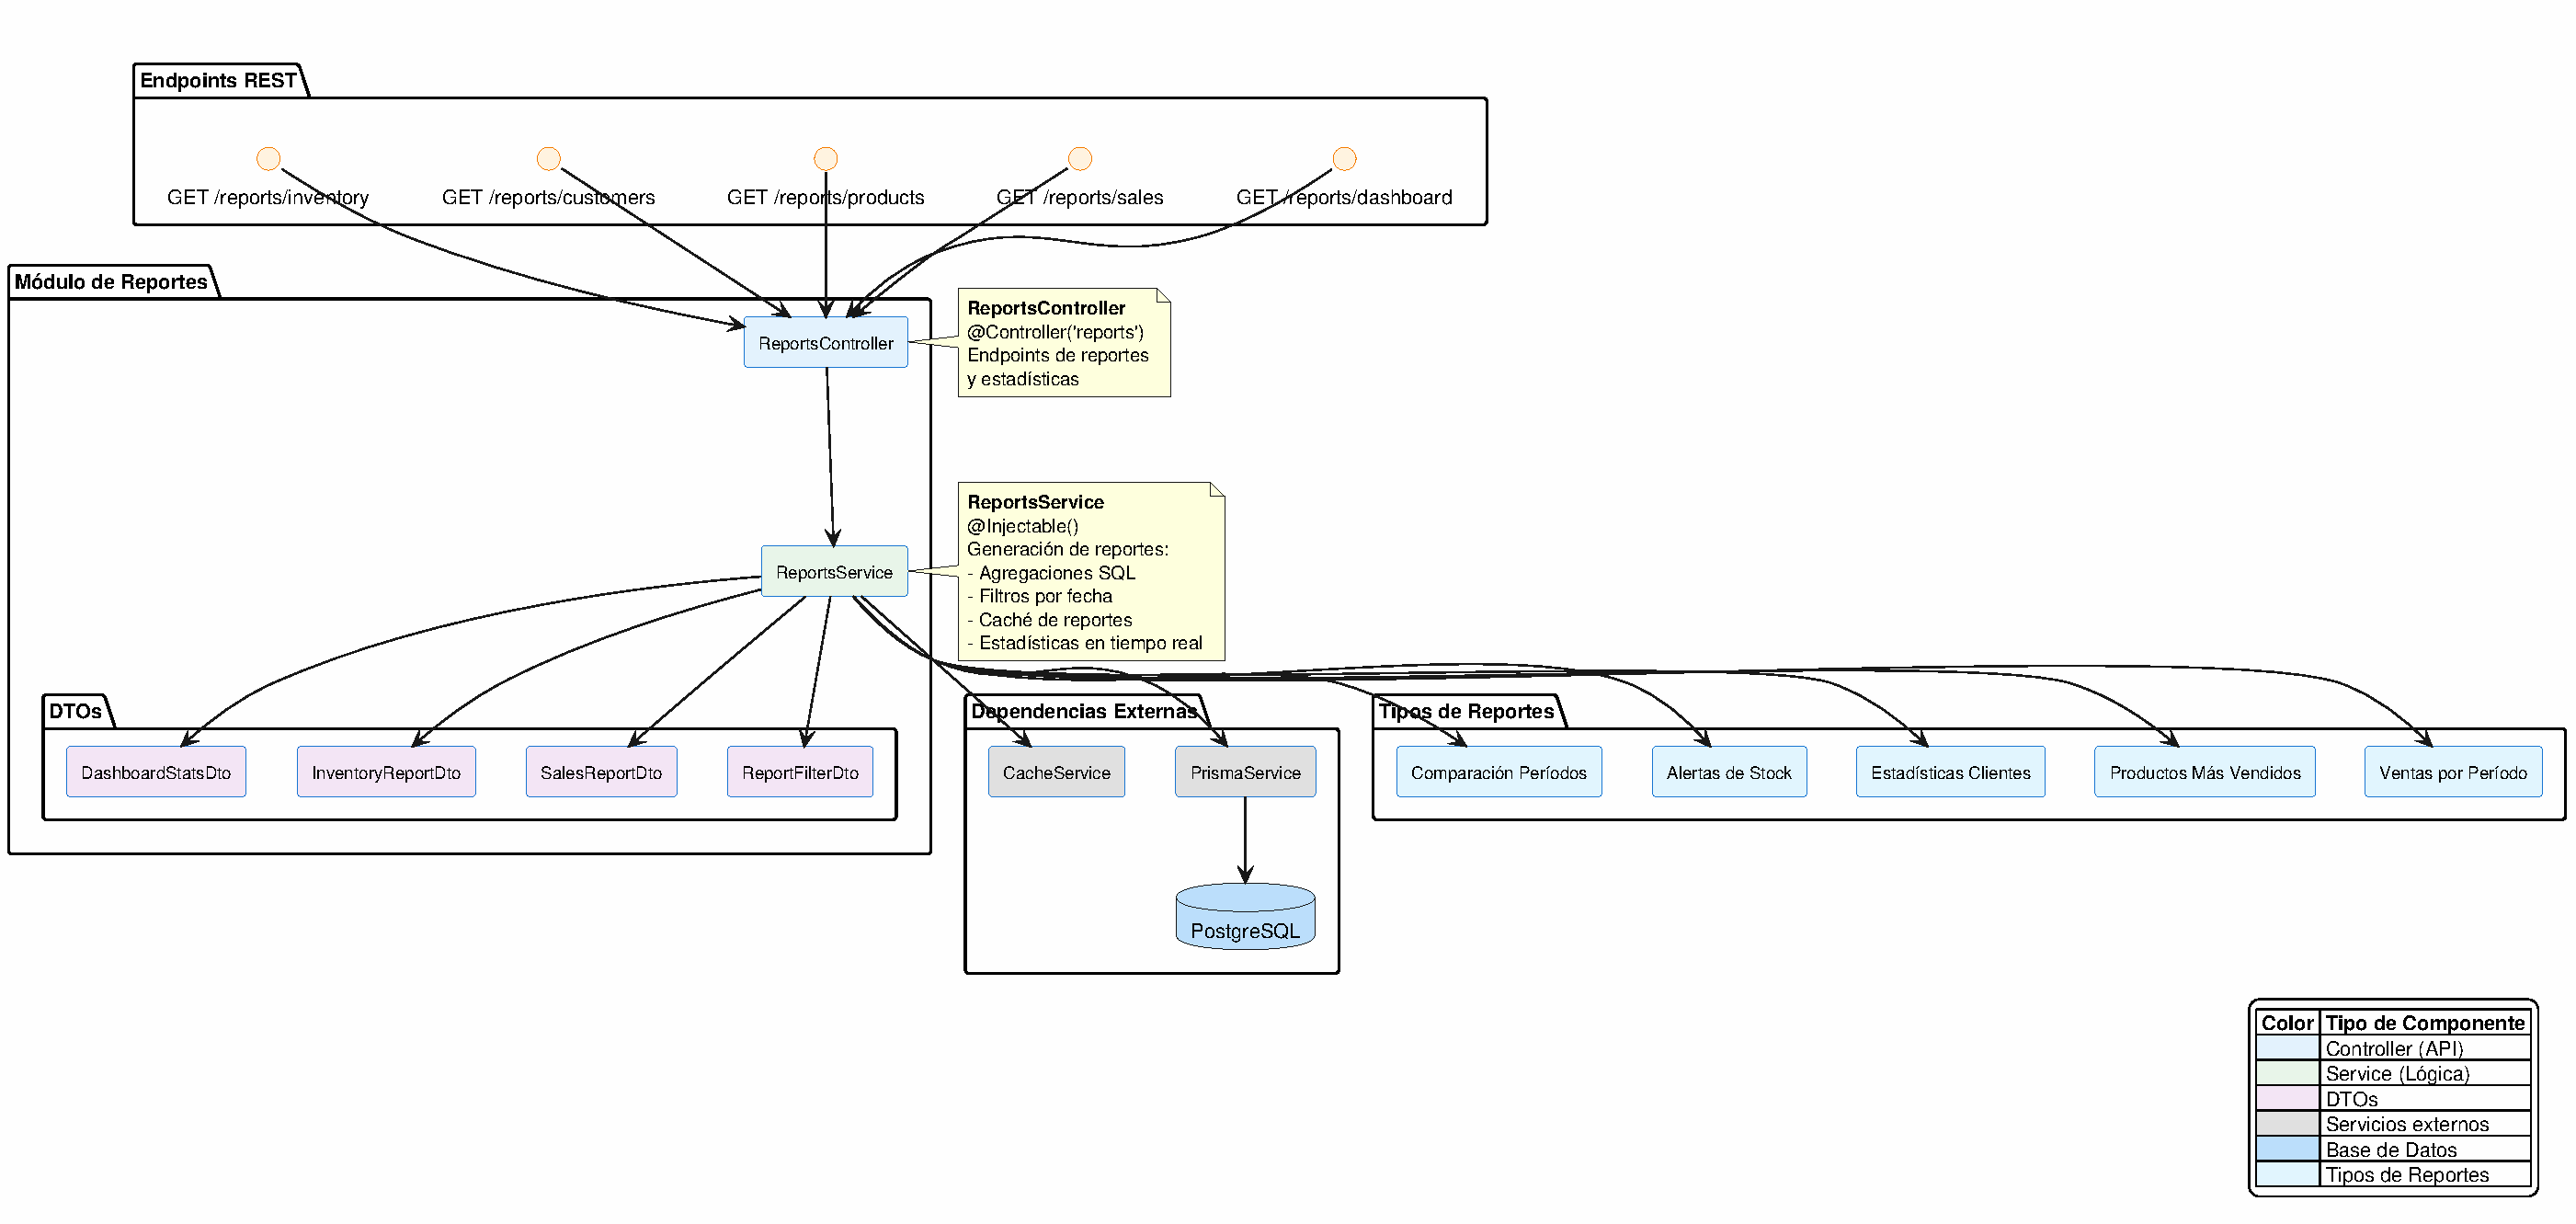
\includegraphics[width=0.85\textwidth]{Images/diagramas-uml/componentes/modulo-reportes}
	\caption{Diagrama de componentes - Módulo de reportes}
	\label{fig:comp-reportes}
\end{figure}

El módulo de exportaciones (Figura \ref{fig:comp-exportaciones}) permite exportar datos en diferentes formatos. El \texttt{ExportsController} expone endpoints para exportar reportes, ventas y productos. El \texttt{ExportsService} genera documentos en PDF, Excel y CSV utilizando librerías especializadas.

\begin{figure}[H]
	\centering
	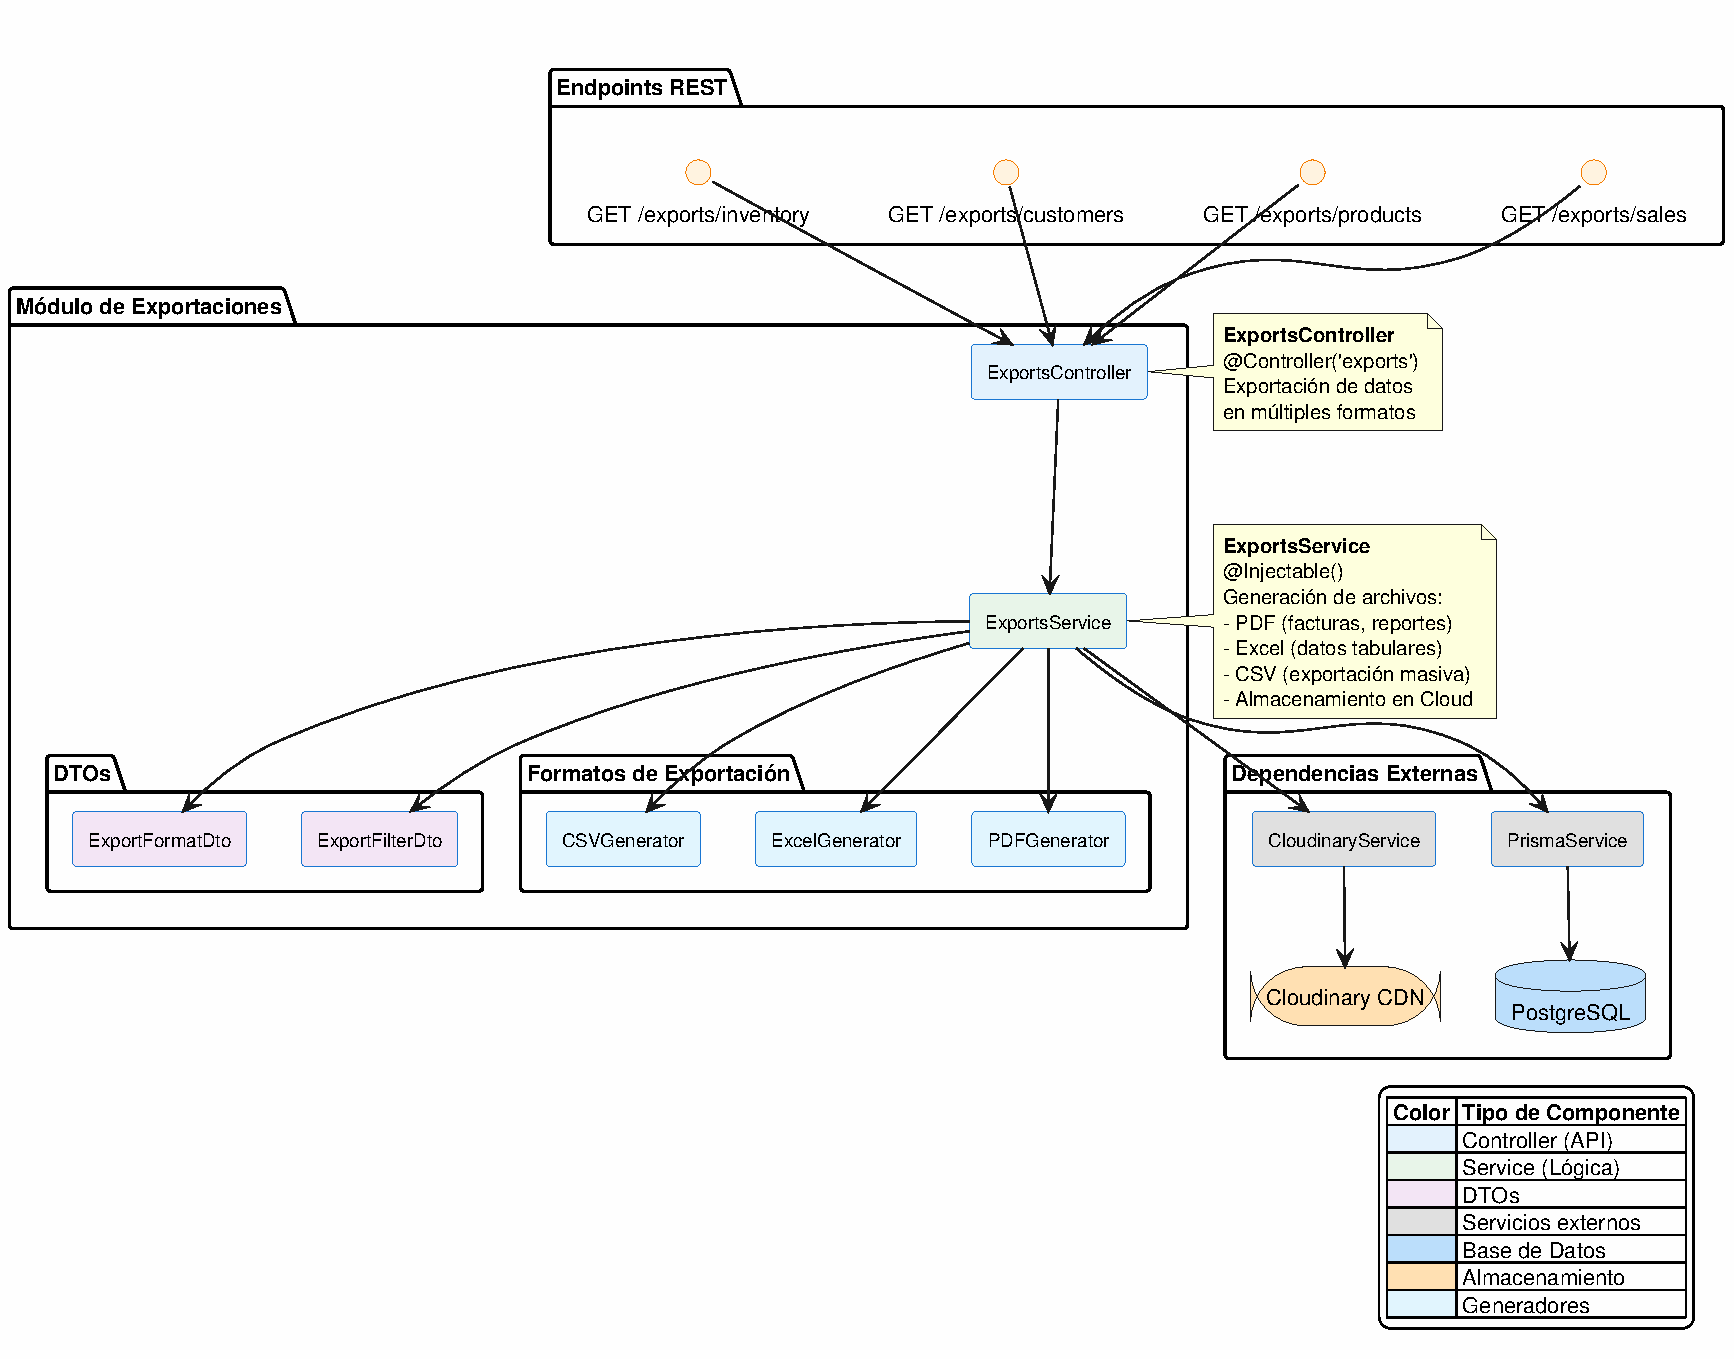
\includegraphics[width=0.85\textwidth]{Images/diagramas-uml/componentes/modulo-exportaciones}
	\caption{Diagrama de componentes - Módulo de exportaciones}
	\label{fig:comp-exportaciones}
\end{figure}

El módulo de configuración (Figura \ref{fig:comp-configuracion}) permite a los administradores gestionar el sistema. El \texttt{SettingsController} expone endpoints para gestión de usuarios, roles, y configuraciones del negocio.

\begin{figure}[H]
	\centering
	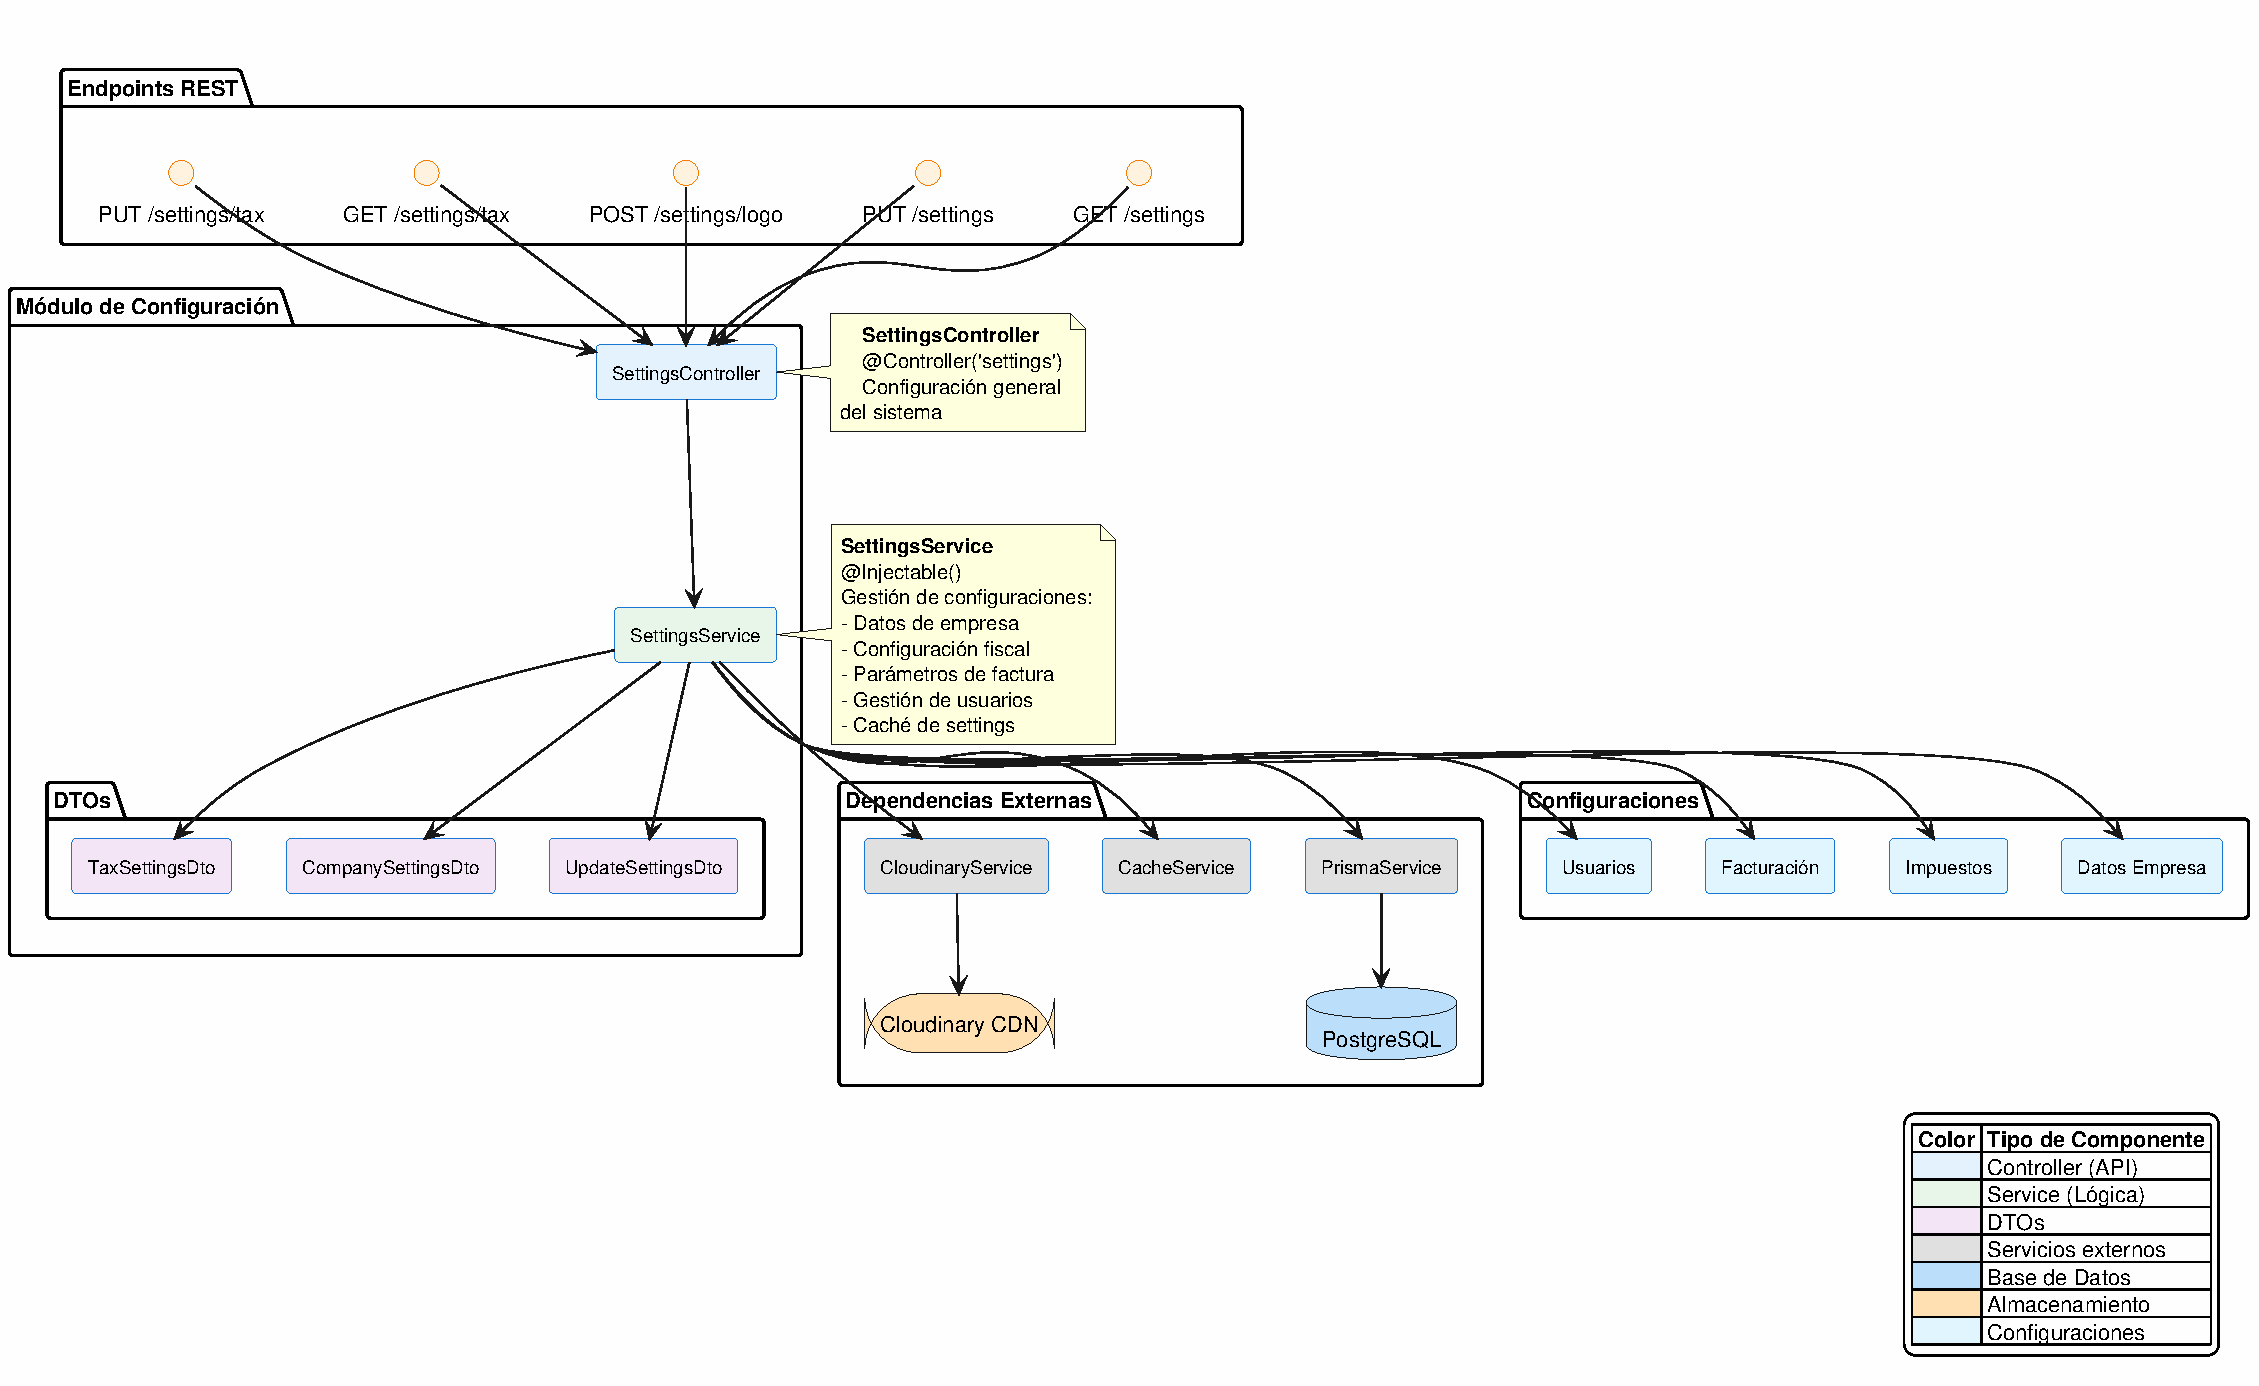
\includegraphics[width=0.85\textwidth]{Images/diagramas-uml/componentes/modulo-configuracion}
	\caption{Diagrama de componentes - Módulo de configuración}
	\label{fig:comp-configuracion}
\end{figure}

El módulo de categorías (Figura \ref{fig:comp-categorias}) gestiona la organización jerárquica de productos. El \texttt{CategoriesController} expone endpoints para CRUD de categorías y subcategorías. El \texttt{CategoriesService} implementa la lógica de negocio incluyendo validaciones de integridad referencial.

\begin{figure}[H]
	\centering
	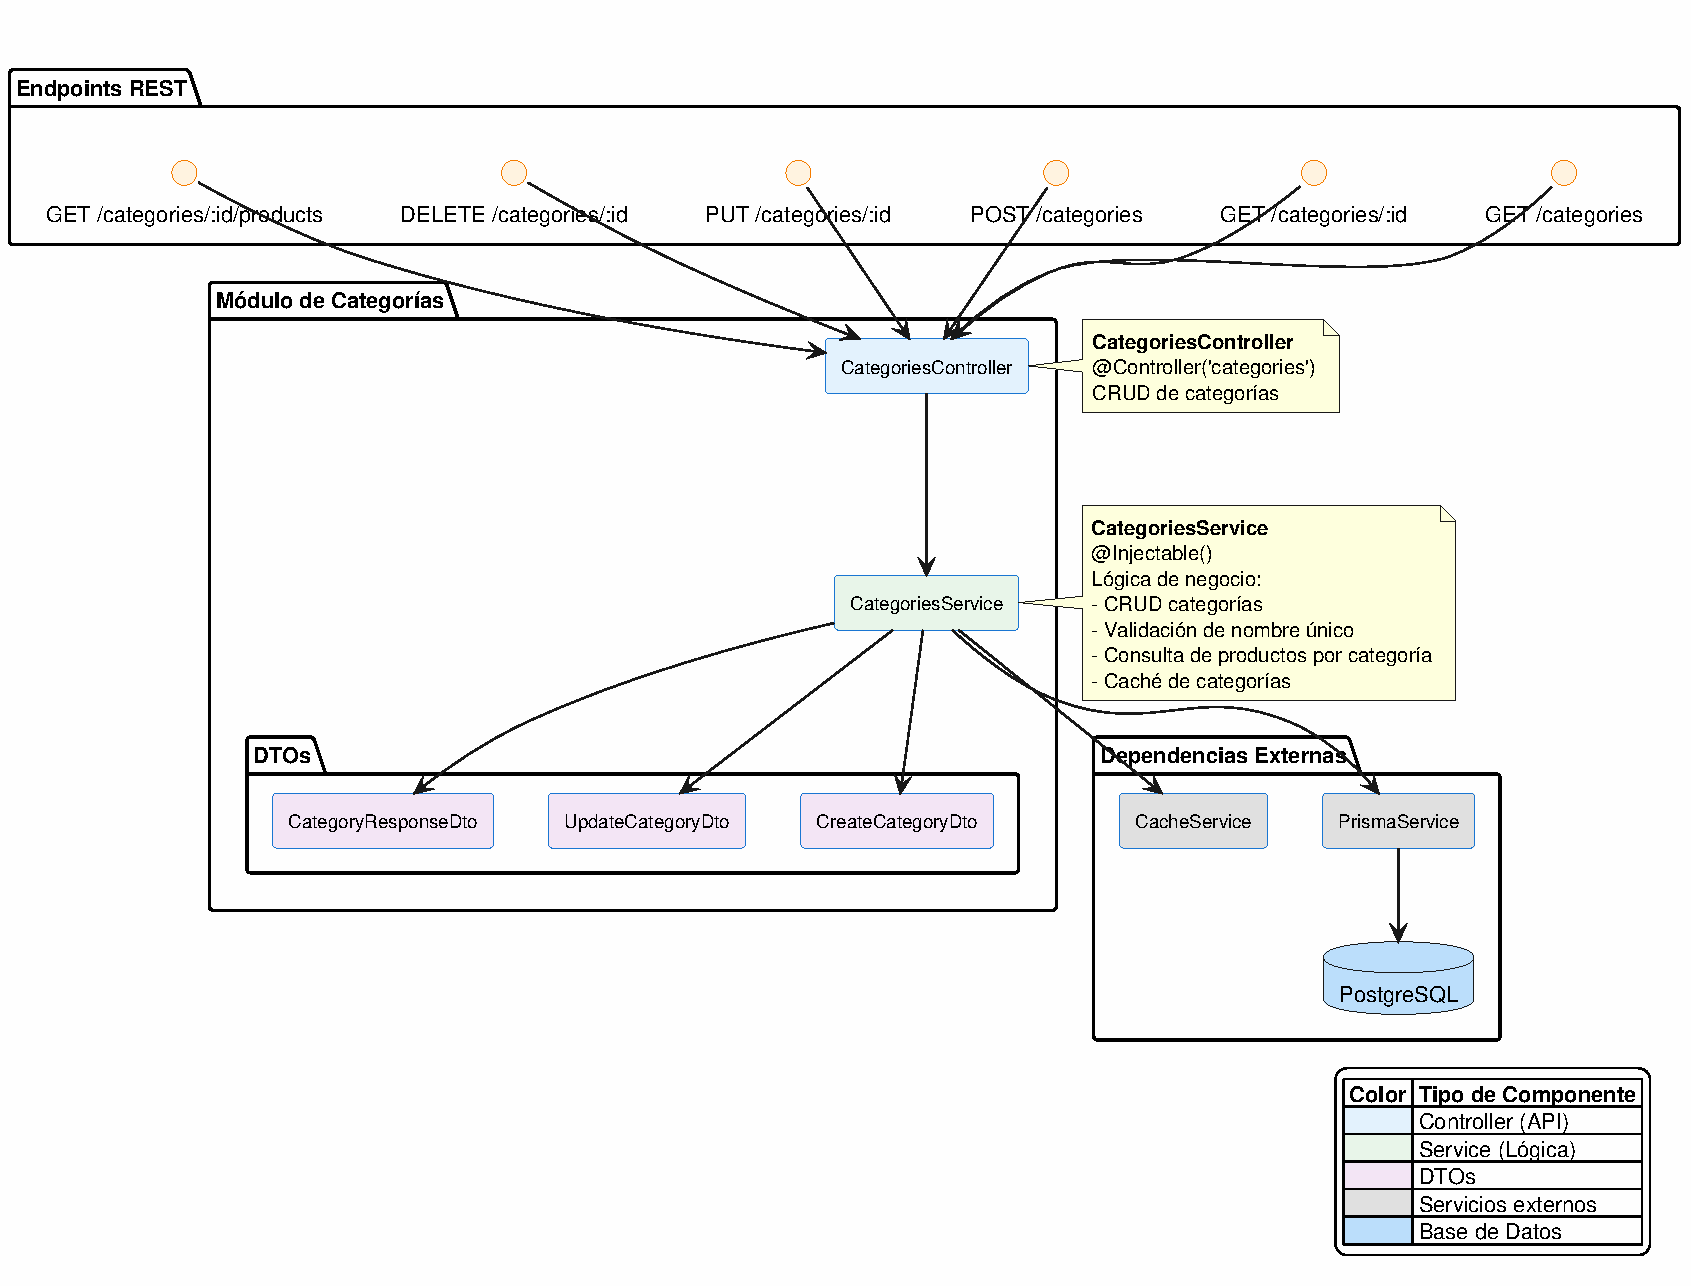
\includegraphics[width=0.85\textwidth]{Images/diagramas-uml/componentes/modulo-categorias}
	\caption{Diagrama de componentes - Módulo de categorías}
	\label{fig:comp-categorias}
\end{figure}

\subsection{Resumen del diseño}

El diseño del sistema se fundamenta en los siguientes principios arquitectónicos:

\textbf{Arquitectura Modular:} El backend está organizado en módulos independientes (auth, products, sales, customers, reports, settings) que pueden desarrollarse, probarse y mantenerse de manera aislada. Cada módulo sigue el patrón Controller-Service-Repository, proporcionando clara separación de responsabilidades.

\textbf{API REST:} La comunicación entre frontend y backend se realiza mediante una API RESTful que utiliza los métodos HTTP estándar (GET, POST, PUT, DELETE) para operaciones sobre recursos identificados con URLs semánticas.

\textbf{Transacciones ACID:} Las operaciones críticas como las ventas implementan transacciones ACID (Atomicidad, Consistencia, Aislamiento, Durabilidad) que garantizan la integridad de datos incluso ante fallos del sistema o errores durante la ejecución.

\textbf{Seguridad por Roles:} El sistema implementa control de acceso basado en roles (RBAC) mediante guards de NestJS. Los roles estan claramente definidos (ADMIN, CASHIER, INVENTORY\_USER) con permisos especificos para cada modulo.

\textbf{Optimización de Rendimiento:} El módulo de reportes implementa caché de resultados para evitar consultas repetitivas a la base de datos, mejorando significativamente el rendimiento de peticiones frecuentes de métricas y estadísticas.

\textbf{Auditoría Completa:} Todas las operaciones críticas del sistema incluyen logging y auditoría que permiten rastrear quién realizó cada acción, cuándo se ejecutó, y qué cambios se aplicaron, proporcionando trazabilidad completa para control interno y compliance.

Este diseño garantiza un sistema robusto, escalable, mantenible y seguro, apropiado para las necesidades de pequeños negocios que requieren gestión integrada de inventario, ventas, clientes y reportes.
